%%%%%%%%%%%%%%%%%%%%%%%%%%%%%%%%%%%%%%%%%%%%%%%%%%%%%%%%%%%%%%%%%%%%%%
% Lớp 11 | Hàm số mũ và hàm số lôgarít | Hàm số mũ. Hàm số lôgarít
% Dạng 1D6?3-2: Tập xác định của hàm số
% Số câu: 170  (sinh tự động bởi tach_cau.py; từ nay thầy sửa trực tiếp file này)
%%%%%%%%%%%%%%%%%%%%%%%%%%%%%%%%%%%%%%%%%%%%%%%%%%%%%%%%%%%%%%%%%%%%%%

%%%%%%%%%%%%%%%% TRẮC NGHIỆM 4 PHƯƠNG ÁN %%%%%%%%%%%%%%%%

% nguồn: Ok_Toan11_TracNghiem_Lan2
\begin{ex}%[1D6N3-2]%[ma:0df598a8]
	Tập xác  định của hàm số $y=\log_2(x-1)^2$ là
	 \choice
		 {$(-1;+\infty)$}
		{\True  $\mathbb{R}\setminus \left\{1\right\}$}
		{$\mathbb{R}$} 
		 {$(1;+\infty)$}
	\loigiai{ 
		Điều kiện xác định $(x-1)^2>0\Leftrightarrow x\ne  1$.\\
		Vậy tập xác định của hàm số đã cho  là
		$\mathscr{D}=\mathbb{R}\setminus  \left\{1\right\}$.
	} 
\end{ex}

% nguồn: Ok_Toan11_TracNghiem_Lan2
\begin{ex}%[1D6N3-2]%[ma:bcfeacdc]
	Tập xác định của  hàm số $y=\log_2(3-x)$ là
	\choice 
		{$(-\infty;+\infty)$} 
		 {$(3;+\infty)$}
		{$\left(-\infty;3\right]$} 
		 {\True $(-\infty;3)$}
	 \loigiai{
		Điều kiện xác định $3-x> 0 \Leftrightarrow x< 3$.  \\
		Tập xác định $\mathscr{D}=(-\infty; 3)$. 
	} 
\end{ex}

% nguồn: Ok_Toan11_TracNghiem_Lan2
\begin{ex}%[1D6N3-2]%[ma:4b07cd67]
	Tập xác định  của hàm số $y=8^x$ là
	\choice 
		{\True  $\mathbb{R}$}
		{$\left[0;+\infty\right)$} 
		{$(0;+\infty)$} 
		{$\mathbb{R}\setminus  \left\{0\right\}$}
	 \loigiai{
		Hàm số $y=8^x$ có tập  xác định là $\mathbb{R}$.
	 }
\end{ex}

% nguồn: Ok_Toan11_TracNghiem_Lan2
\begin{ex}%[1D6N3-2]%[ma:aa773781]
	Tìm tập xác định của  hàm số $y=\log_3(x+3)$.
	 \choice
		{\True $\mathscr{D}=(-3;+\infty)$} 
		 {$\mathscr{D}=\left[-3;+\infty\right)$}
		{$\mathscr{D}=(0;+\infty)$} 
		{$\mathscr{D}=\mathbb{R}\setminus  \left\{-3\right\}$}
	 \loigiai{
		Hàm số xác định khi và chỉ khi $x+3>0\Leftrightarrow x>-3$.  \\
		Vậy tập xác định của  hàm số $\mathscr{D}=(-3;+\infty)$.
	 }
\end{ex}

% nguồn: Ok_Toan11_TracNghiem_Lan2
\begin{ex}%[1D6N3-2]%[ma:faa7aa78]
	Có  bao nhiêu số nguyên thuộc tập xác định của hàm số $y=\ln (15-x^2)$?
	\choice 
		 {\True $7$}
		 {$6$}
		 {$5$}
		 {$8$}
	\loigiai{ 
		Điều kiện $15-x^2>0\Leftrightarrow -\sqrt{15}<x<\sqrt{15}$.  \\
		Do $x\in \mathbb{Z}\Rightarrow x=\left\{\pm  3;\pm 2;\pm 1;0\right\}$.
	 }
\end{ex}

% nguồn: Ok_Toan11_TracNghiem_Lan2
\begin{ex}%[1D6N3-2]%[ma:f36a7ee1]
	Tập xác định của hàm số $y=\log_32x$  là
	\choice 
		 {$(-\infty;0)$}
		 {\True $(0;+\infty)$}
		{$\mathbb{R}$} 
		 {$(1;+\infty)$}
	 \loigiai{
		Hàm số $y=\log_32x$ xác định khi $2x>0\Leftrightarrow  x>0$.
	 }
\end{ex}

% nguồn: Ok_Toan11_TracNghiem_Lan2
\begin{ex}%[1D6N3-2]%[ma:835384a4]
	Tập xác định $\mathscr{D}$  của hàm số $y=\log x^4$ là
	\choice 
		 {$\mathscr{D}=(0;+\infty)$}
		{$\mathscr{D}=(-\infty;0)$} 
		 {$\mathscr{D}=\mathbb{R}$}
		 {\True $\mathscr{D}=\mathbb{R}\setminus \left\{0\right\}$}
	 \loigiai{
		Điều kiện xác định $x^4>0\Leftrightarrow  x\ne 0$.\\
		Vậy tập xác định của  hàm số là $\mathscr{D}=\mathbb{R}\setminus \left\{0\right\}$.
	 }
\end{ex}

% nguồn: Ok_Toan11_TracNghiem_Lan2
\begin{ex}%[1D6N3-2]%[ma:7d284e0f]
	Tập xác định  của hàm số $ y=\log_2(x-1)$ là
	\choice 
		{$\mathbb{R}\setminus\{1\}$} 
		{$[1;+\infty)$} 
		{\True  $(1;+\infty)$}
		{$(-\infty;1)$} 
	\loigiai{ 
		Điều kiện $x-1>0\Leftrightarrow  x>1$.\\
		Tập xác định  của hàm số đã cho là $\mathscr{D}=(1;+\infty)$.
	} 
\end{ex}

% nguồn: Ok_Toan11_TracNghiem_Lan2
\begin{ex}%[1D6N3-2]%[ma:c2a1f1b0]
	Tập  xác định của hàm số $y=\log_{0,5}(x+1)$ là
	\choice 
		{\True $\mathscr{D}=(-1;+\infty)$} 
		 {$\mathscr{D}=\mathbb{R}\setminus \left\{-1\right\}$}
		 {$\mathscr{D}=(0;+\infty)$}
		 {$\mathscr{D}=(-\infty;-1)$}
	\loigiai{ 
		Hàm số $\log_{0,5}(x+1)$ xác định khi và chỉ khi  $x+1>0\Leftrightarrow x>-1$.\\
		Vậy tập xác định của  hàm số là $\mathscr{D}=(-1;+\infty)$.
	 }
\end{ex}

% nguồn: Ok_Toan11_TracNghiem_Lan2
\begin{ex}%[1D6N3-2]%[ma:43eace3e]
	Tập xác định của hàm số $y=\left(\sqrt{3}\right)^x$ là 
	\choice 
		{\True  $\mathbb{R}$}
		{$\left[0;+\infty\right)$} 
		{$\mathbb{R}\setminus  \{0\}$}
		{$(0;+\infty)$} 
	\loigiai{ 
		Tập xác định hàm số  $y=\left(\sqrt{3}\right)^x$ là $\mathbb{R}$.
	} 
\end{ex}

% nguồn: Ok_Toan11_TracNghiem_Lan2
\begin{ex}%[1D6N3-2]%[ma:e8e541e9]
	 Tập xác định của hàm số $y=5^{x+1}+12$ là
	\choice 
		{$[0;+\infty)$} 
		{$\mathbb{R}\setminus  \{0\}$}
		 {\True $\mathbb{R}$}
		{$(0;+\infty)$} 
	\loigiai{ 
		Tập xác  định của hàm số $ y=a^x$ là $\mathbb{R}$.
	 }
\end{ex}

% nguồn: Ok_Toan11_TracNghiem_Lan2
\begin{ex}%[1D6N3-2]%[ma:1c5f55d9]
	 Hàm số $y=(x-1)^{2\,022}$ có tập xác định là
	 \choice
		{\True  $\mathscr{D}=\mathbb{R}$}
		 {$ \mathscr{D}=[1;+\infty)$}
		{$ \mathscr{D}=(1;+\infty)$} 
		{$\mathscr{D}=\mathbb{R}\setminus \{1\}$} 
	\loigiai{ 
		Ta có $y=x-1$ xác định trên và $2\,022$ là số nguyên dương nên hàm số đã cho có tập  xác định là $\mathscr{D}=\mathbb{R}$.
	} 
\end{ex}

% nguồn: Ok_Toan11_TracNghiem_Lan2
\begin{ex}%[1D6N3-2]%[ma:656be2e3]
	 Tập xác định của hàm số $\ln{(x-1)^2}$ là
	 \choice
		{\True  $\mathscr{D}=\mathbb{R}\setminus \left\{1\right\}$}
		{$\mathscr{D}=(1;+\infty)$} 
		{$\mathbb{R}$} 
		 {$\mathscr{D}=\left[1;+\infty\right)$}
	 \loigiai{
		Điều kiện hàm số có nghĩa  là $(x-1)^2>0\Leftrightarrow x\ne 1$.\\
		Vậy tập xác định của hàm  số là $\mathscr{D}=\mathbb{R}\setminus \left\{1\right\}$.
	 }
\end{ex}

% nguồn: Ok_Toan11_TracNghiem_Lan2
\begin{ex}%[1D6N3-2]%[ma:8dc47f9d]
	Tập xác  định của hàm số $y=\ln (x-2)+\sqrt{9-x}$ là
	\choice 
		 {$\left[9;+\infty\right)$}
		 {$\left[2;9\right]$}
		{$(2;9)$} 
		{\True $\left(2;9\right]$} 
	\loigiai{ 
		Ta có điều kiện xác định  của hàm số
		$\heva{&x-2>0 \\&9-x\ge 0} 
		\Leftrightarrow  x\in \left(2;9\right]$.
	 }
\end{ex}

% nguồn: Ok_Toan11_TracNghiem_Lan2
\begin{ex}%[1D6N3-2]%[ma:581c2a11]
	Tập xác  định của hàm số $y=\ln x$ là
	\choice 
		{\True  $(0;+\infty)$}
		{$\mathbb{R}$} 
		{$\left[0;+\infty\right)$} 
		{$\mathbb{R}\setminus \left\{0\right\}$} 
	\loigiai{ 
		Hàm  số $y=\ln x$ có tập xác định là $\mathscr{D}=(0;+\infty)$.
	} 
\end{ex}

% nguồn: Ok_Toan11_TracNghiem_Lan2
\begin{ex}%[1D6N3-2]%[ma:88f0aee9]
	Tập xác định của hàm  số $y=\log (x-1)$ là
	\choice 
		{$[-1;+\infty)$} 
		{\True  $(1;+\infty)$}
		{$[1;+\infty)$} 
		{$(-1;+\infty)$} 
	 \loigiai{
		Hàm số xác  định khi $x-1>0\Leftrightarrow x>1$.
	 }
\end{ex}

% nguồn: Ok_Toan11_TracNghiem_Lan2
\begin{ex}%[1D6N3-2]%[ma:76107870]
	Tập  xác định của hàm số $y=\log_2(x-2)$ là
	\choice 
		{\True  $(2;+\infty)$}
		 {$\left[2;\left. +\infty\right)\right.$}
		 {$(-\infty;2)$}
		 {$\mathbb{R}$}
	 \loigiai{
		Điều  kiện: $x-2>0\Leftrightarrow x>2$.\\
		Vậy tập xác  định của hàm số $y=\log_2(x-2)$ là $(2;+\infty)$.
	} 
\end{ex}

% nguồn: Ok_TracNghiemLop11_Lan1
\begin{ex}%[1D6N3-2]%[ma:1ca15dec]
	Tập xác định của hàm số $y=5^x$ là 
	\choice 
		{\True  $\mathbb{R}$}
		 {$\left(0;+\infty\right)$}
		{$\mathbb{R}\setminus  \left\{0\right\}$}
		 {$\left[0;+\infty\right)$}
	\loigiai{ 
	Tập  xác định của hàm số $y=5^x$ là $\mathbb{R}$.}
\end{ex}

% nguồn: Ok_TracNghiemLop11_Lan1
\begin{ex}%[1D6N3-2]%[ma:9acda642]
	Tập  xác định của hàm số $y=\log_2x$ là
	 \choice
		{$[0;+\infty)$} 
		 {$(-\infty;+\infty)$}
		{\True  $(0;+\infty)$}
		{$\left[2;+\infty\right)$} 
	 \loigiai{
		Điều kiện xác định của hàm số $y=\log_2x$  là $x>0$.\\
		Vậy tập xác định của hàm  số $y=\log_2x$ là $\mathscr{D}=(0;+\infty)$.
	 }
\end{ex}

% nguồn: Ok_TracNghiemLop11_Lan1
\begin{ex}%[1D6N3-2]%[ma:074a91ff]
	Tất cả  các giá trị của $x$ để biểu thức $\log_2(x-1)$ xác định là
	\choice 
		{\True  $x \in(1;+\infty)$}
		{$x \in(-\infty;  1)$}
		{$x \in \mathbb{R} \setminus\{1\}$} 
		 {$x \in(-1;+\infty)$}
	\loigiai{ 
		Biểu thức $\log_2(x-1)$ xác định khi và chỉ  khi $x-1>0\Leftrightarrow x>1$.
	} 
\end{ex}

% nguồn: Ok_TracNghiemLop11_Lan1
\begin{ex}%[1D6N3-2]%[ma:ff4426c0]
	Tập xác định $\mathscr{D}$ của hàm số  $y=\log _2(3 x-6)$ là
	\choice 
		 {\True $\mathscr{D}=(2;+\infty)$}
		{$\mathscr{D}=[2;+\infty)$} 
		 {$\mathscr{D}=(-2;+\infty)$}
		{$\mathscr{D}=(-\infty;  2)$}
	\loigiai{ 
		Điều  kiện: $3 x-6>0\Leftrightarrow x>2$.\\
		Vậy tập xác định của hàm số là $\mathscr{D}=(2;+\infty)$. 
	} 
\end{ex}

% nguồn: Ok_TracNghiemLop11_Lan1
\begin{ex}%[1D6N3-2]%[ma:b473cc77]
	Hàm số $y=2024^x$ có tập xác định  là
	\choice 
		{$\mathbb{R}\setminus  \{0\}$}
		{$[0;+\infty)$} 
		{\True $\mathbb{R}$} 
		 {$(0;+\infty)$}
	\loigiai{ 
		Hàm số $y=2024^x$  có tập xác định là $\mathbb{R}$.
	} 
\end{ex}

% nguồn: Ok_TracNghiemLop11_Lan1
\begin{ex}%[1D6N3-2]%[5-CTST]%[ma:181c1544]
	Tập xác định của hàm số $y  = \log_{4}{x}$ là
	 \choice
		{$\left(-\infty; 0 \right)$} 
		 {$\left[0; +\infty\right)$}
		{\True $\left(0; +\infty\right)$} 
		{$\left(-\infty; +\infty\right)$} 
	\loigiai{ 
		 Điều kiện $x > 0$ do đó $\mathscr{D} = \left(0; +\infty\right)$.
	} 
\end{ex}

% nguồn: Ok_TracNghiemLop11_Lan1
\begin{ex}%[1D6N3-2]%[ma:ed4ec930]
	Tập xác định  của hàm số $y={\log }_2x$ là
	\choice 
		 {$\mathscr{D}=\left[0;+\infty \right)$}
		{$\mathscr{D}=\left(  -\infty;+\infty \right)$}
		{\True $\mathscr{D}=\left(  0;+\infty \right)$}
		{$\mathscr{D}=\left[2;+\infty \right)$} 
	 \loigiai{
		Điều  kiện xác định của hàm số $y={\log }_2x$ là $x>0$.\\
		Vậy tập xác định của hàm số  $y={\log }_2x$ là $\mathscr{D}=\left( 0;+\infty \right).$
	} 
\end{ex}

% nguồn: Ok_TracNghiemLop11_Lan1
\begin{ex}%[1D6N3-2]%[ma:a0b05fc0]
	Tập xác định của hàm số  $y=\log_3 \left(x-4\right)$ là
	\choice 
		 {$\left(5;+\infty \right)$}
		 {$\left(-\infty;+\infty \right)$}
		 {\True $\left(4;+\infty \right)$}
		 {$\left(-\infty;4\right)$}
	\loigiai{ 
		 Điều kiện $x-4> 0\Leftrightarrow x > 4$.\\
		Tập xác định  $\mathscr{D}=\left(4;+\infty \right)$.
	} 
\end{ex}

% nguồn: Ok_TracNghiemLop11_Lan1
\begin{ex}%[1D6N3-2]%[ma:ec1f622b]
	Tập xác định của hàm số $  y=\log_{10} x $ là
	 \choice
		{$ (-\infty;+\infty)  $}
		{$ (-\infty;0) $} 
		 {$ [0;+\infty) $}
		{\True  $ (0;+\infty) $}
	 \loigiai{
		Điều  kiện $ x>0 $.\\
		Tập xác định của hàm số  là $ \mathscr{D}=(0;+\infty) $.
	} 
\end{ex}

% nguồn: Ok_TracNghiemLop11_Lan1
\begin{ex}%[1D6N3-2]%[ma:1401b499]
	 Tập xác định của hàm số $y=\log 2024x$ là
	\choice 
		{\True  $\mathscr{D}=(0;+\infty)$}
		{$\mathscr{D}=[0;+\infty)$} 
		 {$\mathscr{D}=\mathbb{R}$}
		{$\mathscr{D}=(2024;+\infty)$} 
	 \loigiai{
		Điều kiện xác định của hàm số là  $2024x>0\Leftrightarrow x>0$.\\
		Vậy  tập xác định của hàm số là $\mathscr{D}=(0;+\infty)$.
	} 
\end{ex}

% nguồn: Ok_TracNghiemLop11_Lan1
\begin{ex}%[1D6N3-2]%[ma:b61598c9]
	Tập xác định của  hàm số $y=2^x$ là
	 \choice
		 {\True $\mathbb{R}$}
		{$\left(0;+\infty \right)$} 
		 {$\left[0;+\infty \right)$}
		{$\mathbb{R}\setminus \{0\}$} 
	 \loigiai{
		Hàm số mũ $y=2^x$ xác  định với mọi $x\in \mathbb{R}$ nên tập xác định là $\mathscr{D}=\mathbb{R}$.
	} 
\end{ex}

% nguồn: Ok_TracNghiemLop11_Lan1
\begin{ex}%[1D6N3-2]%[ma:67f3bf95]
	Tập xác định  của hàm số $y=\log_3x$ là
	 \choice
		{$(-\infty;0)$} 
		 {\True $(0;+\infty)$}
		 {$(-\infty;+\infty)$}
		{$[0;+\infty)$} 
	 \loigiai{
		Điều kiện xác định của hàm số $y=\log_3x$ là  $x > 0$.
	} 
\end{ex}

% nguồn: Ok_TracNghiemLop11_Lan1
\begin{ex}%[1D6N3-2]%[ma:76610cb5]
	Tập xác  định của hàm số $y=2^x$ là
	\choice 
		 {\True $\mathbb{R}$}
		 {$(0;+\infty)$}
		 {$[0;+\infty)$}
		{$R \backslash\{0\}$} 
	\loigiai{ 
		Tập xác định của  hàm số $y=2^x$ là $\mathbb{R}$.
	} 
\end{ex}

% nguồn: Ok_TracNghiemLop11_Lan1
\begin{ex}%[1D6N3-2]%[ma:a0855129]
	Tìm tập xác định $\mathscr{D}$ của hàm  số $y=2018^{\sqrt{2-x^2}}$.
	\choice 
		 {$\mathscr{D}=\left(-\sqrt{2};\sqrt{2}\right]$}
		 {$\mathscr{D}=\left(-\sqrt{2};\sqrt{2}\right)$}
		{\True $\mathscr{D}=\left[-\sqrt{2};\sqrt{2}\right]$} 
		 {$\mathscr{D}=\left(-\infty;\sqrt{2}\right]$}
	\loigiai{ 
		Điều kiện: $2-x^2\geq 0\Leftrightarrow -\sqrt{2}\leq x  \leq \sqrt{2}$.\\
		Tập xác  định $\mathscr{D}=\left[-\sqrt{2};\sqrt{2}\right]$.
	} 
\end{ex}

% nguồn: Ok_TracNghiemLop11_Lan1
\begin{ex}%[1D6N3-2]%[ma:0dfa31f3]
	Tập xác định của hàm số $y=\log_5x$  là
	 \choice
		 {$\left[0;+\infty\right)$}
		 {$\left(- \infty; 0\right)$}
		{\True $\left(0;+\infty\right)$} 
		{$\left(- \infty;+\infty\right)$} 
	 \loigiai{
		Hàm số $y=\log_5x$ xác định khi và chỉ khi $x>0$. \\ 
		Tập  xác định của hàm số là $\mathscr{D}=\left(0;+\infty\right)$.
	} 
\end{ex}

% nguồn: Ok_TracNghiemLop11_Lan1
\begin{ex}%[1D6N3-2]%[ma:5fcde1a1]
	Tập xác định  của hàm số $y=4^x$ là
	 \choice
		{$\mathbb{R}\setminus\{0\}$} 
		 {$[0;+\infty)$}
		 {$(0;+\infty)$}
		{\True $\mathbb{R}$} 
	\loigiai{ 
	Ta có hàm số mũ $y=4^x$ luôn  xác định với mọi $x\in\mathbb{R}$.}
\end{ex}

% nguồn: Ok_TracNghiemLop11_Lan1
\begin{ex}%[1D6N3-2]%[ma:3c930cc9]
	 Tập xác định của hàm số $y=\log_3 \left(2x+1\right)$ là
	\choice 
		 {$\left(-\infty;\dfrac{1}{2}\right)$}
		{ $\left(\dfrac{1}{2};+\infty\right)$} 
		{$\left(0;+\infty\right)$} 
		{\True $\left(-\dfrac{1}{2};+\infty\right)$} 
	 \loigiai{
	Hàm số $y=\log_3 \left(2x+1\right)$ xác định khi và  chỉ khi $2x+1>0 \Leftrightarrow x>-\dfrac{1}{2}$.\\
	Vậy tập xác định của hàm  số là $\mathscr{D} = \left(-\dfrac{1}{2};+\infty\right)$.
	 }
\end{ex}

% nguồn: Ok_TracNghiemLop11_Lan1
\begin{ex}%[1D6N3-2]%[ma:147e1f1c]
	Tập  xác định của hàm số $ y={{\log }_5}x$ là
	\choice 
		 { $[0;+\infty)$}
		{ $( -\infty;0)$} 
		 {\True $( 0;+\infty)$}
		{ $( -\infty;+\infty)$} 
	\loigiai{ 
		Hàm số xác định: $ x>0$.\\ 
	Tập xác định: $D=( 0;+\infty)$.} 
\end{ex}

% nguồn: Ok_TracNghiemLop11_Lan1
\begin{ex}%[1D6N3-2]%[ma:9945dee4]
	Tập  xác định của hàm số $y=5^x$ là
	\choice 
		{\True  $\mathbb{R}$}
		 {$(0;+\infty)$}
		 {$\mathbb{R}\setminus \{0\}$}
		{$[0;+\infty)$} 
	 \loigiai{
		Tập xác định của hàm số $y=5^x$  là $\mathbb{R}$.
	} 
\end{ex}

% nguồn: Ok_TracNghiemLop11_Lan1
\begin{ex}%[1D6N3-2]%[ma:fcc55a84]
	 Tập xác định của hàm số $y=\log_3(x-1)$ là
	 \choice
		 {\True $(1;+\infty)$}
		 {$(-\infty;1)$}
		{$[1;+\infty)$} 
		{$(-\infty;+\infty)$} 
	\loigiai{ Điều kiện xác định $x-1>0\Leftrightarrow  x>1$.\\
	Tập xác định  của hàm số là $\mathscr{D}=(1;+\infty)$.}
\end{ex}

% nguồn: Ok_TracNghiemLop11_Lan1
\begin{ex}%[1D6N3-2]%[ma:c1746dd4]
	Cho hàm số $y=3^x$. Tập xác  định của hàm số là?
	\choice 
		{$(0;+\infty)$} 
		{$(-\infty;0)$} 
		{\True  $\mathbb{R}$}
		{$(3;+\infty)$} 
	\loigiai{Tập xác định của $y=3^x$ là $\mathscr{D}=\mathbb{R}$. 
	 }
\end{ex}

% nguồn: Ok_TracNghiemLop11_Lan1
\begin{ex}%[1D6N3-2]%[ma:f13a8946]
	Tập xác định của hàm số  $y=\left(\dfrac{2023}{2024}\right)^x$ là
	\choice 
		{$\mathbb{R}\setminus\{0\}$} 
		{$(0;+\infty)$} 
		{\True  $\mathbb{R}$}
		 {$[0;+\infty)$}
	\loigiai{ 
	Hàm số $y=\left(\dfrac{2023}{2024}\right)^x$ có tập xác định  là $\mathscr{D}=\mathbb{R}$.
	} 
\end{ex}

% nguồn: Ok_TracNghiemLop11_Lan1
\begin{ex}%[1D6N3-2]%[ma:619ece23]
	Tập xác định của  hàm số $y=\log_2x$ là
	 \choice
		 {$[0;+\infty)$}
		 {$(-\infty;+\infty)$}
		{\True  $(0;+\infty)$}
		{$[2;+\infty)$} 
	 \loigiai{
		Điều kiện $x>0$.\\ 
		Tập xác định của hàm số là $\mathscr{D}=(0;+\infty)$. 
	} 
\end{ex}

% nguồn: Ok_TracNghiemLop11_Lan1
\begin{ex}%[1D6N3-2]%[ma:92954d1e]
	Tập xác định của hàm số $y=(x+1)^{\tfrac{2}{3}}$ là 
	\choice 
		 {$[-1;+\infty)$}
		{\True  $(-1;+\infty)$}
		 {$(0;+\infty)$}
		{$\mathbb{R}  \setminus\{-1\}$}
	 \loigiai{
		 Điều kiện xác định $x+1>0 \Leftrightarrow x>-1$. \\
		 Tập xác định $\mathscr{D}=(-1;+\infty)$.
	} 
\end{ex}

% nguồn: Ok_TracNghiemLop11_Lan1
\begin{ex}%[1D6N3-2]%[ma:501e545f]
	Tập xác định của  hàm số $y=\mathrm{e}^x$ là
	\choice 
		{$(0;+\infty)$} 
		 {\True $\mathbb{R}$}
		 {$(\mathrm{e};+\infty)$}
		{$\mathbb{R} \setminus\{0\}$} 
	\loigiai{ 
		Hàm số $y=\mathrm{e}^x$  xác định với mọi $x\in\mathbb{R}$.
	} 
\end{ex}

% nguồn: Ok_TracNghiemLop11_Lan1
\begin{ex}%[1D6N3-2]%[ma:5340d44c]
	Tập xác định của hàm số $y=a^x$ $(a>0,~ a \ne 1)$ là 
	\choice 
		 {$\mathscr{D}=(0;+\infty)$}{$\mathscr{D}=\mathbb{R}\setminus\{1\}$}{$\mathscr{D}=[0;+\infty)$}{\True $\mathscr{D}=\mathbb{R}$}
	\loigiai{ 
		Tập xác định  của hàm số $y=a^x$ $(a>0,~ a \ne 1)$ là $\mathscr{D}=\mathbb{R}$.
	 }
\end{ex}

% nguồn: Ok_TracNghiemLop11_Lan1
\begin{ex}%[1D6N3-2]%[ma:d0ba59b5]
	Tập xác định của  hàm số $y=\log_a x$ là
	\choice 
		 { $\left[0;+\infty\right)$}
		{\True $\left(0;+\infty\right)$} 
		{$\left(-\infty;0\right)$} 
		{$\left(-\infty;+\infty\right)$} 
	 \loigiai{
		Điều kiện: $x>0$.\\ 
	 Vậy tập xác định của hàm số đã cho là $\mathscr{D}=\left(0;+\infty\right)$.}
\end{ex}

% nguồn: Ok_TracNghiemLop11_Lan1
\begin{ex}%[1D6N3-2]%[ma:664fc73b]
	Tập xác định của hàm số $y=\log _{2024}(x-2023)$ là 
	\choice 
		 {\True $(2023;+\infty)$}
		 {$[2023;+\infty)$}
		{$(-2023;+\infty)$} 
		{$(-\infty;-2023)$} 
	\loigiai{ 
		Hàm  số đã cho xác định khi $x-2023>0\Leftrightarrow x>2023$.\\
		Vậy $\mathscr{D}=(2023;+\infty)$. 
	} 
\end{ex}

% nguồn: Ok_Toan11_TracNghiem_Lan2
\begin{ex}%[1D6H3-2]%[ma:861e4d7e]
	Có bao  nhiêu số nguyên thuộc tập xác định của hàm số $y=\log[(6-x)(x+2)]$?
	 \choice
		{\True $7$} 
		 {$8$}
		{$9$} 
		{Vô số} 
	 \loigiai{
		Điều kiện $(6-x)(x+2)>0 \Leftrightarrow  -2<x<6$.\\
		Tập xác định của  hàm số là
		 $\mathscr{D}=(-2;6)$.\\
		Vậy có $7$ số nguyên  thuộc tập xác định $\mathscr{D}$ là $-1;0;1;2;3;4;5$.
	 }
\end{ex}

% nguồn: Ok_Toan11_TracNghiem_Lan2
\begin{ex}%[1D6H3-2]%[ma:47af5d19]
	 Tất cả các giá trị thực của tham số $m$ để hàm số $y=\log\left(x^2-2x-m+1\right)$ có tập xác định là $\mathbb{R}$.
	 \choice
		 {$m\ge 0$}
		 {\True $m<0$}
		{$m\le  2$}
		 {$m>2$}
	\loigiai{ 
		Điều kiện $x^2-2x-m+1>0$.\\ 
		Để  hàm số có tập xác định là $\mathbb{R}$ khi và chỉ khi
		\allowdisplaybreaks 
		\begin{eqnarray*}
			x^2-2x-m+1>0,\,\forall x\in\mathbb{R}&\Leftrightarrow&  (-1)^2-\left(-m+1\right)<0\\
			 &\Leftrightarrow&m<0.
		\end{eqnarray*}
	} 
\end{ex}

% nguồn: Ok_Toan11_TracNghiem_Lan2
\begin{ex}%[1D6H3-2]%[ma:2b6d03b9]
	Tập xác định của hàm số $y=(x-2\,021)^{\tfrac{2\,019}{2\,021}}$ là 
	 \choice
		 {$(-2021;+\infty)$}
		{$\mathbb{R}\setminus \{2\,021\}$} 
		{\True  $(2\,021;+\infty)$}
		 {$(-\infty;2\,021)$}
	 \loigiai{
		Điều  kiện $x-2021>0\Leftrightarrow x>2\,021$.\\
	Vậy  tập xác định của hàm số là $\mathscr{D}=(2\,021;+\infty)$ .}
\end{ex}

% nguồn: Ok_Toan11_TracNghiem_Lan2
\begin{ex}%[1D6H3-2]%[ma:a0aa3bda]
	Tập xác  định của hàm số $ y=x^{\tfrac{3}{2}}$ là
	 \choice
		 {\True $(0;+\infty)$}
		{$(2;+\infty)$} 
		 {$\mathbb{R}$}
		{$\mathbb{R}\setminus\{0\}$} 
	\loigiai{ 
		Tập xác định của  hàm số $y=x^{\tfrac{3}{2}}$ là $(0;+\infty)$.
	 }
\end{ex}

% nguồn: Ok_Toan11_TracNghiem_Lan2
\begin{ex}%[1D6H3-2]%[ma:823890f8]
	Tập xác định của hàm số  $y=\dfrac{1}{\log_2x-1}$ là
	\choice 
		{$\mathbb{R}\setminus  \{2\}$}
		 {$(0;+\infty)$}
		 {\True $(0;+\infty)\setminus\{2\}$}
		{$(0;+\infty)\setminus  \{1\}$}
	\loigiai{ 
		 Hàm số xác định khi $\heva{&
		x>0\\& 
		\log_2x-1\ne 0} \Leftrightarrow \heva{& 
		 x>0\\&
		\log_2x\ne 1}  \Leftrightarrow\heva{&
		 x>0\\&
		x\ne 2.}$\\ 
	Vậy tập xác định  $\mathscr{D}=(0;+\infty)\setminus\{2\}$.}
\end{ex}

% nguồn: Ok_Toan11_TracNghiem_Lan2
\begin{ex}%[1D6H3-2]%[ma:874c87fc]
	Tập  xác định của hàm số $y=\log x$ là
	 \choice
		 {$[1;+\infty)$}
		{\True  $(0;+\infty)$}
		{$[0;+\infty)$} 
		 {$(1;+\infty)$}
	 \loigiai{
		Hàm số $y=\log x$ xác định $\Leftrightarrow  x>0$.\\
	Vậy tập xác định của hàm số là $\mathscr{D}=(0;+\infty)$.} 
\end{ex}

% nguồn: Ok_Toan11_TracNghiem_Lan2
\begin{ex}%[1D6H3-2]%[ma:485034f6]
	Tập xác định $ \mathscr{D}$ của hàm số $y=(x-3)^{-5}+\log_3(4-x)$ là 
	\choice 
		{$\mathscr{D}=(3;\,4)$} 
		{\True  $\mathscr{D}=(-\infty;4)\setminus\{3\}$}
		 {$\mathscr{D}=(4;+\infty)$}
		{$\mathscr{D}=(-\infty;4)$} 
	\loigiai{ 
		 Hàm số đã cho xác định khi: $\heva{& x-3\ne 0\\&4-x>0} \Leftrightarrow\heva{&
		x\ne 3\\& 
		 x<4.}$\\
		Tập xác định  của hàm số đã cho là $ \mathscr{D}=(-\infty;4)\setminus \{3\}$.
	 }
\end{ex}

% nguồn: Ok_Toan11_TracNghiem_Lan2
\begin{ex}%[1D6H3-2]%[ma:64a8010b]
	Tập xác định $\mathscr{D}$ của hàm  số $y=\ln(1-x)$ là
	 \choice
		{$\mathscr{D}=\mathbb{R}\setminus\{1\}$} 
		{$\mathscr{D}=\mathbb{R}$} 
		{\True $\mathscr{D}=(-\infty;1)$} 
		{$\mathscr{D}=(1;+\infty)$} 
	\loigiai{ 
		Hàm số xác định  $\Leftrightarrow 1-x>0\Leftrightarrow x<1$.
	 }
\end{ex}

% nguồn: Ok_Toan11_TracNghiem_Lan2
\begin{ex}%[1D6H3-2]%[ma:26ca6c5b]
	Tìm tập xác định của hàm số $y=\ln(3-x)+x^\pi$. 
	\choice 
		 {$(-\infty;3]$}
		 {$(0;+\infty)$}
		 {$(-\infty;3)$}
		{\True $(0;3)$} 
	\loigiai{ 
		Hàm số có xác định khi $\heva{&3-x>0\\ 
		 &x>0} \Leftrightarrow 0<x<3$.
	 }
\end{ex}

% nguồn: Ok_Toan11_TracNghiem_Lan2
\begin{ex}%[1D6H3-2]%[ma:88854511]
	Tập xác định của hàm số $ y=\sqrt{2-\ln x}$ là 
	\choice 
		{\True  $\left(0;\mathrm{e^2}\right]$}
		 {$\left(-\infty;\mathrm{e^2}\right)$}
		 {$\left(-\infty;\mathrm{e^2}\right]$}
		 {$\left[\mathrm{e^2};+\infty\right)$}
	 \loigiai{
		Hàm số xác định  $\Leftrightarrow\heva{&
		2-\ln  x\ge 0\\&
		 x>0} \Leftrightarrow\heva{&
		\ln  x\le 2\\&
		 x>0} \Leftrightarrow\heva{&
		x\le \mathrm{e^2}\\& 
		x>0.}$\\ 
		Vậy  tập xác định $ \mathscr{D}=\left(0;\mathrm{e^2}\right]$.
	 }
\end{ex}

% nguồn: Ok_Toan11_TracNghiem_Lan2
\begin{ex}%[1D6H3-2]%[ma:df905e9f]
	Tập xác  định của hàm số $ y=\sqrt{\log_{\tfrac{1}{2}}(x^2+7x)+3}$ là
	\choice 
		{$(-8;-7)\cup(0;1)$} 
		{\True  $[-8;-7)\cup(0;1]$}
		{$[-8;-7)\cup(0;1)$} 
		 {$[-8;-7]\cup(0;1]$}
	\loigiai{ 
		Hàm số đã  cho xác định khi và chỉ khi
		\begin{eqnarray*}
			 &&\heva{&x^2+7x>0 \\&\log _{\tfrac{1}{2}}(x^2+7x)+3 \ge 0} \Leftrightarrow \heva{&x^2+7x>0 \\&x^2+7x \le \left(\dfrac{1}{2}\right)^{-3}}\\
			&\Leftrightarrow &\heva{&x^2+7x>0 \\& x^2+7x-8\le 0} \Leftrightarrow\heva{&\hoac{&x>0\\& x<-7} \\&-8\le x\le 1}\\ 
			&\Leftrightarrow&\hoac{&-8\le x<-7\\& 0<x\le 1.} 
		\end{eqnarray*}
		Vậy tập xác định của  hàm số là $\mathscr{D}=[-8;-7)\cup(0;1]$.
	} 
\end{ex}

% nguồn: Ok_Toan11_TracNghiem_Lan2
\begin{ex}%[1D6H3-2]%[ma:3ef18263]
	Tập xác định $\mathscr{D}$ của hàm số  $y=\dfrac{1}{\sqrt{\log_3\dfrac{2x}{x+1}-1}}$ là
	 \choice
		{$\mathscr{D}=(-\infty;-3)$} 
		 {$\mathscr{D}=(-1;+\infty)$}
		{\True $\mathscr{D}=(-3;-1)$} 
		{$ \mathscr{D}=(0;3)$} 
	 \loigiai{
		Hàm số xác định khi và chỉ  khi
		 $$\heva{&
		 \log_3\dfrac{2x}{x+1}>1\\&
		\dfrac{2x}{x+1}>  0} \Leftrightarrow\heva{&
		 \dfrac{2x}{x+1}>3^1\\&
		\dfrac{2x}{x+1}> 0}  \Leftrightarrow\dfrac{2x}{x+1}> 3\Leftrightarrow\dfrac{2x}{x+1}-3>0\Leftrightarrow-3 < x <-1.$$
	Vậy tập xác định của hàm  số là $\mathscr{D}=(-3;-1)$.}
\end{ex}

% nguồn: Ok_Toan11_TracNghiem_Lan2
\begin{ex}%[1D6H3-2]%[ma:bc34133b]
	Tập xác định của  hàm số $y=\dfrac{1}{\log_{2} x-1}$ là
	 \choice
		 {$\mathbb{R}\setminus\left\{2\right\}$}
		{$(0;+\infty)  $}
		{\True $(0;+\infty)\setminus\left\{2\right\}$} 
		{  $(0;+\infty)\setminus\left\{1\right\}$}
	\loigiai{Điều kiện xác định  của hàm số $\heva{& x > 0 \\&\log_{2} x \ne 1} \Leftrightarrow \heva{& x > 0 \\& x \ne 2.}$\\
	Vậy tập xác  định của hàm số là $\mathscr{D}=\left(0;+\infty\right)\setminus\left\{2\right\}$.}
\end{ex}

% nguồn: Ok_Toan11_TracNghiem_Lan2
\begin{ex}%[1D6H3-2]%[ma:9eef5932]
	Tập xác định của hàm số $\log_3(x-4)$  là
	 \choice
		{$(5;+\infty)$} 
		{$(-\infty;+\infty)$} 
		 {\True $(4;+\infty)$}
		{$(-\infty;-4)$} 
	\loigiai{ 
		Hàm số đã  cho xác định khi $x-4>0 \Leftrightarrow x>4$.\\
		Vậy tập xác định của hàm số  là $\mathscr{D}=(4;+\infty)$.
	} 
\end{ex}

% nguồn: Ok_Toan11_TracNghiem_Lan2
\begin{ex}%[1D6H3-2]%[ma:d9653300]
	Tập xác  định của hàm số $y=\log_2(x-1)$ là
	\choice 
		 {$(2;+\infty)$}
		 {$(-\infty;+\infty)$}
		{\True $(1;+\infty)$} 
		 {$(-\infty;1)$}
	\loigiai{ 
		Điều kiện xác định  $x-1>0 \Leftrightarrow x>1$.\\
		Vậy tập xác định của hàm số $y=\log_2(x-1)$ là  $\mathscr{D}=(1;+\infty)$.
	} 
\end{ex}

% nguồn: Ok_Toan11_TracNghiem_Lan2
\begin{ex}%[1D6H3-2]%[ma:3e4f45f0]
	Tìm tập xác định $\mathscr{D}$ của hàm số $  y=x^{\tfrac{1}{3}}+\log_3(1-x)$.
	 \choice
		{$ \mathscr{D}=(0;1]$} 
		 {$ \mathscr{D}=(0;+\infty)$}
		{\True $  \mathscr{D}=(0;1)$}
		{$ \mathscr{D}=(1;+\infty)$} 
	 \loigiai{
		Hàm số xác định $\Leftrightarrow\heva{& 
		 x>0\\&
		1-x>0} \Leftrightarrow  0<x<1$.\\
	Vậy tập xác  định $\mathscr{D}=(0;1)$.}
\end{ex}

% nguồn: Ok_TracNghiemLop11_Lan1
\begin{ex}%[1D6H3-2]%[ma:1c9aaa54]
	Tập xác định của hàm số $f(x)=\log_5\left(30-x^2\right)$  chứa bao nhiêu số nguyên?
	\choice 
		{\True $11$} 
		{$5$} 
		 {$6$}
		 {$10$}
	\loigiai{ 
		Điều  kiện xác định $30-x^2>0\Leftrightarrow -\sqrt{30}<x<\sqrt{30}$.\\
		Vì $x\in \mathbb{Z}$  nên $x\in \left\{-5;-4;-3;\dots;5\right\}$.\\
		Vậy  có $11$ giá trị nguyên $x$ trong tập xác định.
	} 
\end{ex}

% nguồn: Ok_TracNghiemLop11_Lan1
\begin{ex}%[1D6H3-2]%[ma:0bfef2f2]
	 Tập xác định $\mathscr{D}$ của hàm số $y=\log_2(x^2-3x+2)$ là
	 \choice
		 {\True $\mathscr{D}=(-\infty;1)\cup(2;+\infty)$}
		 {$\mathscr{D}=(-\infty;1]\cup[2;+\infty)$}
		 {$\mathscr{D}=(1;2)$}
		 {$\mathscr{D}=[1;2]$}
	\loigiai{Hàm  số xác định khi $x^2-3x+2>0\Leftrightarrow \hoac{&x<1\\&x>2.}$\\
		Vậy tập xác định của hàm số là $\mathscr{D}=(-\infty;1)\cup  (2;+\infty)$.
	 }
\end{ex}

% nguồn: Ok_TracNghiemLop11_Lan1
\begin{ex}%[1D6H3-2]%[ma:e007f5d8]
	Tìm tập xác định $\mathscr{D}$ của hàm  số $y=\log _{2018} \dfrac{x-1}{x+2}$.
	\choice 
		{$\mathscr{D}=[1; +  \infty)$}
		{$\mathscr{D}=( -  2; 1)$}
		{\True $\mathscr{D}=( - \infty; - 2)\cup(1;  + \infty)$}
		{$\mathscr{D}=( - \infty;  - 2)$}
	 \loigiai{
		Điều kiện $\dfrac{x-1}{x+2}>0 \Leftrightarrow x<-2$ hoặc  $x > 1$.
	} 
\end{ex}

% nguồn: Ok_TracNghiemLop11_Lan1
\begin{ex}%[1D6H3-2]%[ma:cced0423]
	Tập  xác định của hàm số $y=\log_2\dfrac{x-2}{3}$ là
	 \choice
		{\True $(2;+\infty)$} 
		 {$(-\infty;2)$}
		 {$(2;+\infty)$}
		{$(2;+\infty)\setminus \{3\}$} 
	 \loigiai{
		 Hàm số xác định khi $x-2>0\Leftrightarrow x>2$.\\
		Vậy tập xác định của hàm số là  $\mathscr{D}=(2;+\infty)$.
	 }
\end{ex}

% nguồn: Ok_TracNghiemLop11_Lan1
\begin{ex}%[1D6H3-2]%[ma:25dd4bd9]
	Tập xác  định của hàm số $y=\log _4x$ là
	\choice 
		 {$(-\infty; 0)$}
		{$[0;+\infty)$} 
		 {\True $(0;+\infty)$}
		 {$(-\infty;+\infty)$}
	\loigiai{ 
		Hàm số $y=\log _4x$ xác định  khi và chỉ khi $4x>0 \Leftrightarrow x>0$. \\
		Vậy tập xác định của hàm số đã cho là  $(0;+\infty)$.
	} 
\end{ex}

% nguồn: Ok_TracNghiemLop11_Lan1
\begin{ex}%[1D6H3-2]%[ma:02ae156f]
	Tập xác  định của hàm số $y=\log_2 \left(x^2-2x-3\right)$ là
	\choice 
		{$\left( -\infty;-1 \right]\cup \left[3;+\infty \right)$} 
		{$\left[-1;3  \right]$}
		{\True $\left(  -\infty;-1 \right)\cup \left( 3;+\infty \right)$}
		{$\left(  -1;3\right)$}
	\loigiai{ 
	Hàm số $y=\log_2 \left(x^2-2x-3\right)$ xác định khi  và chỉ khi $x^2-2x-3>0 \Leftrightarrow \hoac{&x<-1\\&x>3}$.\\
	Vậy tập xác  định của hàm số là $\mathscr{D} = \left( -\infty;-1 \right)\cup \left( 3;+\infty \right)$.
	} 
\end{ex}

% nguồn: Ok_TracNghiemLop11_Lan1
\begin{ex}%[1D6H3-2]%[ma:301b3ed8]
	Hàm số $y=\log_{x-1}2$ xác  định khi và chỉ khi
	 \choice
		{$x>2$} 
		{\True  $\heva{&x>1\\&x\ne 2}$}
		 {$x>1$}
		 {$x\ne 2$}
	\loigiai{ 
		Hàm số $y=\log_{x-1}2$ xác định khi và chỉ khi $\heva{&x-1>0\\&x-1\ne 1}\Leftrightarrow\heva{&x>1\\&x\ne 2.}$ 
	} 
\end{ex}

% nguồn: Ok_TracNghiemLop11_Lan1
\begin{ex}%[1D6H3-2]%[ma:5c6d2157]
	Tìm tập xác định $\mathscr{D}$ của hàm  số $y=(2x-x^2)^{\frac{1}{3}}+\log_2(x-1)^2$.
	\choice 
		 {$\mathscr{D}=(0;2)$}
		 {$\mathscr{D}=(0;1)$}
		{$\mathscr{D}=\mathbb{R}\setminus \{0;2\}$} 
		{\True $\mathscr{D}=(0;2)\setminus \{1\}$} 
	\loigiai{ 
		Điều kiện: $\heva{&2x-x^2>0\\ &(x-1)^2>0}\Leftrightarrow \heva{&0<x<2\\ &x-1\neq 0}\Leftrightarrow \heva{&0<x<2\\&x\neq  1}$.\\
		Tập xác  định $\mathscr{D}=(0;2)\setminus \{1\}$.\\
		\textbf{Cần nhớ: }$A^2>0 \Rightarrow A\neq  0$ và $|A|>0 \Leftrightarrow A\neq 0$.
	 }
\end{ex}

% nguồn: Ok_TracNghiemLop11_Lan1
\begin{ex}%[1D6H3-2]%[ma:765c6e0c]
	Có bao nhiêu số nguyên thuộc tập tập xác định của  hàm số $y=\ln\left(15-x^2\right)$?
	 \choice
		{$5$} 
		{$8$} 
		 {\True $7$}
		{$6$} 
	\loigiai{ 
		Điều kiện $15-x^2>0\Leftrightarrow -\sqrt{15}<x<\sqrt{15}$.\\ 
		Tập xác  định $\mathscr{D}=(-\sqrt{15};\sqrt{15})$.\\
		 Vậy có tất cả $7$ số nguyên thuộc tập tập xác định của hàm số.
	} 
\end{ex}

% nguồn: Ok_TracNghiemLop11_Lan1
\begin{ex}%[1D6H3-2]%[ma:af8e3bda]
	Trong các hàm số sau, hàm số nào \textbf{không} xác  định trên $\mathbb{R}$?
	 \choice
		 {$y=3^x$}
		 {\True $y=\log(x^2)$}
		 {$y=\ln\left(|x|+1\right)$}
		{$y=\left(0{,}3\right)^x$} 
	\loigiai{Hàm số $y=\log(x^2)$ xác  định khi $x^2>0 \Leftrightarrow x \ne 0$.
	} 
\end{ex}

% nguồn: Ok_TracNghiemLop11_Lan1
\begin{ex}%[1D6H3-2]%[ma:307d4228]
	Tìm tập xác định của hàm số $y=\ln  \left(-2x^2+x+3\right)$.
	\choice 
		 {$\mathscr{D}=(-\infty;-1) \cup\left(\dfrac{3}{2};+\infty\right)$}
		 {$\mathscr{D}=\left[-1; \dfrac{3}{2}\right]$}
		 {$\mathscr{D}=(-\infty;-1] \cup\left[\dfrac{3}{2};+\infty\right)$}
		{\True $\mathscr{D}=\left(-1; \dfrac{3}{2}\right)$} 
	 \loigiai{
		Hàm  số xác định khi $-2x^2+x+3>0\Leftrightarrow -1<x<\dfrac{3}{2}$.\\
		Vậy tập xác định của hàm số là $\mathscr{D}=\left(-1; \dfrac{3}{2}\right)$. 
	 }
\end{ex}

% nguồn: Ok_TracNghiemLop11_Lan1
\begin{ex}%[1D6H3-2]%[ma:b9d1ca89]
	Tìm tập xác định của hàm số $y=2^{\sqrt{x}}+\log  \left(3-x\right)$.
	\choice 
		 {$[0;+\infty)$}
		 {$\left(0;3\right)$}
		{$\left(-\infty;3\right)$} 
		{\True  $\left[0;3\right)$}
	\loigiai{ 
		Điều  kiện xác định:
		 $\heva{&x\ge 0 \\&3-x>0}\Leftrightarrow \heva{&x\ge 0 \\&x<3}\Leftrightarrow 0\leq x<3$.\\
		 Vậy tập xác định của hàm số đã cho là $\mathscr{D}=\left[0;3\right)$
	 }
\end{ex}

% nguồn: Ok_TracNghiemLop11_Lan1
\begin{ex}%[1D6H3-2]%[ma:35ff4d52]
	 Có bao nhiêu số nguyên $x>0$ để hàm số $y=\log_{2018}(10-x)$ xác định?
	\choice 
		 {$10$}
		{$2018$} 
		{vô  số}
		 {\True $9$}
	\loigiai{ 
		Hàm  số xác định khi $10-x>0\Leftrightarrow x<10$.\\
		Mà $x>0$ là số nguyên nên $0<x<10$.  Suy ra có $9$ số nguyên cần tìm.
	} 
\end{ex}

% nguồn: Ok_TracNghiemLop11_Lan1
\begin{ex}%[1D6H3-2]%[ma:1862cc69]
	Có bao nhiêu số nguyên thuộc tập xác định của hàm số $y=\log \left[\left(6-x\right)\left(x+2\right)\right]$? 
	 \choice
		{\True $7$} 
		{$8$} 
		{Vô  số}
		 {$9$}
	\loigiai{ 
		Hàm số xác định khi  $\left(6-x\right)\left(x+2\right) > 0\Leftrightarrow-2 < x < 6$.\\
		Vì $x\in \mathbb{Z}\Rightarrow  x\in \left\{-1; 0; 1; 2; 3; 4; 5\right\}$.\\
		Vậy có $7$ số nguyên thuộc  tập xác định của hàm số $y=\log \left[\left(6-x\right)\left(x+2\right)\right]$
	 }
\end{ex}

% nguồn: Ok_TracNghiemLop11_Lan1
\begin{ex}%[1D6H3-2]%[ma:2e4e7322]
	Tập xác định của hàm  số $y=\log_3\left(x-4\right)$ là
	\choice 
		 {$(5;+\infty)$}
		 {$(-\infty;+\infty)$}
		{\True $(4;+\infty)$} 
		 {$(-\infty;4)$}
	 \loigiai{
		Điều  kiện: $x-4>0\Leftrightarrow x>4$.\\
		Tập  xác định: $\mathscr{D}=(4;+\infty)$.
	} 
\end{ex}

% nguồn: Ok_Toan11_TracNghiem_Lan2
\begin{ex}%[1D6V3-2]%[ma:0244357c]
	Tìm tất cả các giá trị thực của tham số $m$ để hàm số  $ y=\mathrm{e}^{\tfrac{1}{\sqrt{x^2+mx+1}}}$ có tập xác định là $\mathbb{R}$.
	 \choice
		{$\hoac{&m <-2\\& 
		m>2}$} 
		{$m>2$} 
		{\True  $-2<m<2$}
		{$  m<2$}
	\loigiai{ 
		Hàm số có tập xác  định là $\mathbb{R}$ khi và chỉ khi
		 $$\Delta < 0 \Leftrightarrow m^2-4< 0 \Leftrightarrow-2<m<2.$$
	 }
\end{ex}

% nguồn: Ok_Toan11_TracNghiem_Lan2
\begin{ex}%[1D6V3-2]%[ma:5fb25c70]
	Tìm tất cả các giá  trị thực của tham số $m$ để hàm số $y=\log_{3} \left(x^2-4x-m+1 \right)$ xác định với mọi $x \in \mathbb{R}$.
	 \choice
		 {\True $m <-3$}
		{$m >  3$}
		{$m  \ge-3$}
		 {$m < 3$}
	\loigiai{Hàm số $y  = \log_{3} \left(x^2-4x-m+1 \right)$ xác định với mọi $x \in \mathbb{R}$ khi và chỉ khi \\
	$x^2-4x-m+1 > 0$, $\forall x \in \mathbb{R}$ $\Leftrightarrow \heva{& a > 0 \\& \Delta' < 0} \Leftrightarrow \heva{& 1 > 0 \\& 4+m-1 <  0} \Leftrightarrow m < -3$.}
\end{ex}

% nguồn: Ok_Toan11_TracNghiem_Lan2
\begin{ex}%[1D6V3-2]%[ma:c466ba32]
	Có tất cả bao nhiêu giá trị nguyên dương của  tham số $m$ để hàm số\break $y=\log_{2} \left(x^2-2x+2\,022-m \right)$ có tập xác định là $\mathbb{R}$?
	\choice 
		 {$2\,022$}
		 {$2\,021$}
		{\True  $2\,020$}
		{$2\,019$} 
	\loigiai{Điều kiện xác định $x^2-2x+2\,022-m >  0$.\\
		Hàm số $y = \log_{2} \left(x^2-2x+2\,022-m \right)$ có tập  xác định là $\mathbb{R}$ khi và chỉ khi $$x^2-2x+2\,022-m > 0, \forall x \in \mathbb{R} \Leftrightarrow \Delta' = 1-(2\,022-m) < 0 \Leftrightarrow m < 2\,021.$$
	Vậy có $2\,020$ giá trị của $m$ thỏa mãn bài toán.} 
\end{ex}

% nguồn: Ok_TracNghiemLop11_Lan1
\begin{ex}%[1D6V3-2]%[ma:3eb2723a]
	Tìm tất cả các giá trị thực  của tham số $m$ để hàm số $y=\log \left(x^2-2 x+m\right)$ có tập xác định là $\mathbb{R}$.
	\choice 
		{$m<1$} 
		{$m \geq  1$}
		{\True $m>1$} 
		{$m  \leq 1$}
	\loigiai{Hàm số $y=\log \left(x^2-2 x+m\right)$ có tập xác định là $\mathbb{R}$ khi  và chỉ khi $x^2-2 x+m>0$ với mọi $x$.\\
	Hay $\heva{&a=1>0\\&\Delta^{'}=\left(-1\right)^2-1\cdot m  <0}\Leftrightarrow m>1$.}
\end{ex}

% nguồn: Ok_TracNghiemLop11_Lan1
\begin{ex}%[1D6V3-2]%[ma:753479e7]
	Số các giá trị nguyên dương của tham số $m$ để hàm số\\ $f(x)=\log_{2024}\left[x^2-2(m-1)x-m^2+3m+8\right]$ xác định với mọi giá trị thực của  $x$.
	\choice 
		 {$4$}
		{$2$} 
		{\True  $3$}
		{$1$} 
	 \loigiai{
		Ta thấy  hàm số $f(x)=\log_{2024}\left[x^2-2(m-1)x-m^2+3m+8\right]$ xác định với mọi giá trị thực của $x$ khi và chỉ khi $x^2-2(m-1)x-m^2+3m+8>0,\forall x\in\mathbb{R}$ \\
		 $ \Leftrightarrow\heva{&1>0\\&\Delta’=(m-1)^2-\left(-m^2+3m+8\right)<0}\Leftrightarrow 2m^2-5m-7<0\Leftrightarrow-1<m<\dfrac{7}{2}$. \\
		Do $m\in\mathbb{N}^*$ nên  $m\in\{1;2;3\}$.\\
	Vậy có $3$ giá trị  nguyên dương của tham số $m$ thoả mãn yêu cầu bài toán.}
\end{ex}

% nguồn: Ok_TracNghiemLop11_Lan1
\begin{ex}%[1D6V3-2]%[ma:456183a3]
	Số giá trị nguyên của tham số  $m \in(-2024; 2024)$ để hàm số $y=\left(x^{2}-2 x-m+1\right)^{\sqrt{5}}$ xác định với $\forall x \in \mathbb{R}$ là
	\choice 
		{$4048$} 
		{$2024$} 
		{\True $2023$} 
		{Vô số} 
	\loigiai{ 
		 Cần nhớ với $f(x)=a x^2 + b x + c$ ($a\ne 0$) thì $f(x) > 0$ với mọi $x\in\mathbb{R}$ khi và chỉ khi xảy ra một trong hai trường hợp:
		\begin{itemize}
			\item $a>0$ và  $\Delta<0$;
			\item  $a = 0$, $b=0$, $c>0$.
		\end{itemize}
		Hàm số  xác định khi và chỉ khi $x^2 - 2x - m + 1>0$.\\
		Để $\mathscr{D}=\mathbb{R}$ thì $x^2 - 2x - m  + 1>0$ luôn đúng với $\forall x\in\mathbb{R}$, điều này tương đương với
		\[ 
		\heva{&a=1>0\\&\Delta=4 - 4(-m + 1)<0}\Leftrightarrow  m<0.
		 \]
		Kết hợp với $m\in\mathbb{Z}$ và $m \in (  - 2024; 2024)$ nên $m\in\{ - 2023;\ldots; - 1\}$. \\
		Vậy có  $2023$ số nguyên $m$ thoả mãn.
	 }
\end{ex}

% nguồn: Ok_TracNghiemLop11_Lan1
\begin{ex}%[1D6K3-2]%[ma:9cbe2a3d]
	Tìm tất cả các giá trị của $m$ để hàm số $y=\ln\left(-x^2+mx+2m+1\right)$  xác định với mọi $x\in(1;2)$.
	 \choice
		{$m\ge-\dfrac{1}{3}$} 
		{\True  $m\ge\dfrac{3}{4}$}
		 {$m >\dfrac{3}{4}$}
		{$m  <-\dfrac{1}{3}$}
	\loigiai{ 
		Hàm số xác  định với mọi $x\in(1;2)$ khi và chỉ khi
		\allowdisplaybreaks 
		\begin{eqnarray*}
			 &&-x^2+mx+2m+1 > 0,\,\forall x\in(1;2)\\
			&\Leftrightarrow& f(x)=x^2-mx-2m-1  < 0,\,\forall x\in\left(1;2\right)\\
			&\Rightarrow& f(x)=0 \text{ có 2 nghiệm thỏa mãn } x_1\le 1 < 2\le{x_2}\\ 
			&\Rightarrow&\heva{&f(1)\le 0\\&f(2)\le  0}\\
			&\Leftrightarrow& \heva{&-3m\le 0\\&-4m+3\le 0}  \\
			&\Leftrightarrow& m\ge\dfrac{3}{4}. 
		\end{eqnarray*}
	} 
\end{ex}

% nguồn: Ok_TracNghiemLop11_Lan1
\begin{ex}%[1D6K3-2]%[ma:29167898]
	Tìm giá trị  nguyên lớn nhất của tham số $m$ để hàm số $y=\dfrac{1}{\sqrt{\log_3\left(x^2-2mx+17\right)}}$ có tập xác định $\mathbb{R}$.
	 \choice
		 {\True $3$}
		 {$8$}
		 {$9$}
		{$7$} 
	\loigiai{ 
		Hàm số $y=\dfrac{1}{\sqrt{\log_3\left(x^2-2mx+17\right)}}$ có tập xác định  $\mathbb{R}$
		 \allowdisplaybreaks
		\begin{eqnarray*}
			&\Leftrightarrow&  \heva{&x^2-3mx+17>0,\,\forall x\in\mathbb{R}\\&\log_3\left(x^2-2mx+17\right)>0,\,\forall x\in\mathbb{R}}\\
			 &\Leftrightarrow& x^2-2mx+17 > 1,\,\forall x\in\mathbb{R}\\
			&\Leftrightarrow& x^2-2mx+16  > 0,\,\forall x\in\mathbb{R}\\
			&\Leftrightarrow&  \Delta ' < 0\Leftrightarrow m^2-16 < 0\Leftrightarrow-4 < m < 4.
		\end{eqnarray*}
		Vậy giá trị nguyên lớn nhất của tham số $m$ là  $3$.
	} 
\end{ex}

% nguồn: Ok_TracNghiemLop11_Lan1
\begin{ex}%[1D6K3-2]%[ma:8520a30d]
	Tìm tất cả các giá trị của tham số $m$ để hàm số $y=\log\left(x^2+2x+11\right)+m$ có giá trị nhỏ nhất bằng $5$. 
	 \choice
		{$m=1$} 
		{$m\in\mathbb{R}$} 
		{$m > 1$} 
		 {\True $m=4$}
	 \loigiai{
		$y=\log\left(x^2+2x+11\right)+m=\log\left[\left(x+1\right)^2+10\right]+m\ge 1+m$.\\ 
		Hàm số $y=\log\left(x^2+2x+11\right)+m$ có  giá trị nhỏ nhất bằng $5$ thì $1+m=5\Leftrightarrow m=4$.
	 }
\end{ex}

% nguồn: Ok_TracNghiemLop11_Lan1
\begin{ex}%[1D6K3-2]%[ma:9b22886e]
	Hàm số $y=\ln\left(x^2+mx+1\right)$ xác định với mọi giá  trị của $x$ khi
	\choice 
		 {$\hoac{&m<-2\\&m>2}$}
		 {$m>2$}
		{\True $-2<m<2$} 
		{$m<2$} 
	\loigiai{ 
		Yêu cầu bài toán $\Leftrightarrow x^2+mx+1>0,\,\forall \in\mathbb{R}  \Leftrightarrow x^2-4<0 \Leftrightarrow -2<m<2$.
	} 
\end{ex}

% nguồn: Ok_TracNghiemLop11_Lan1
\begin{ex}%[1D6K3-2]%[ma:5d79cebb]
	Tìm tất cả các giá trị của  $m$ để hàm số $y=\ln\left(x^2+2mx+3m-2\right)$ xác định với mọi $x\in\mathbb{R}$.
	\choice 
		 {$m > 2$}
		{\True $1 < m <  2$}
		{$m < 1$} 
		{$m <-\dfrac{1}{3}$} 
	 \loigiai{
		Hàm số xác định với mọi $x\in\mathbb{R}$ khi  $x^2+2mx+3m-2$, $x\in\mathbb{R}$.\\
		$\Rightarrow\heva{&a > 0\\&\Delta  ' < 0} \Leftrightarrow\heva{&1 > 0\\&m^2-3m+2 < 0} \Leftrightarrow 1 < m < 2$.
	} 
\end{ex}

% nguồn: Ok_TracNghiemLop11_Lan1
\begin{ex}%[1D6K3-2]%[ma:c4b1a6aa]
	Tìm tất cả các giá trị thực của tham số $m$ để hàm số $y=\ln\left(x^2-2x+m+1\right)$ có tập xác định  là $\mathbb{R}$.
	 \choice
		{$0 < m  < 3$}
		{\True $m > 0$} 
		{$\hoac{&m <-1\\&m  > 0}$}
		{$m=0$} 
	 \loigiai{
		Hàm số $y=\ln\left(x^2-2x+m+1\right)$ xác định  trên $\mathbb{R}$ khi và chỉ khi
		\allowdisplaybreaks 
		\begin{eqnarray*}
			&&  x^2-2x+m+1>0,\,\forall x\in\mathbb{R}\\
			 &\Leftrightarrow& \Delta '=1-m-1 < 0\\
			&\Leftrightarrow&  m > 0.
		\end{eqnarray*}
	 }
\end{ex}

% nguồn: Ok_TracNghiemLop11_Lan1
\begin{ex}%[1D6K3-2]%[ma:7926ab99]
	Tìm tập giá trị của hàm số $f(x)=2+\log_2x$  trên đoạn $\left[2;4\right]$.
	 \choice
		 {$T=\left[1;3\right]$}
		{$T=\left[0;2\right]$} 
		 {\True $T=\left[3;4\right]$}
		{$T=\left[2;4\right]$} 
	 \loigiai{
		 Ta có
		\allowdisplaybreaks 
		\begin{eqnarray*}
			&&2\le  x\le 4\\
			&\Leftrightarrow&  \log_2 2\le{\log_2}x\le{\log_2}4\\
			&\Leftrightarrow&  2+\log_22\le 2+\log_2x\le 2+\log_24\\
			 &\Leftrightarrow& 3\le f(x)\le 4.
		\end{eqnarray*}
		Vậy $T=\left[3;4\right]$. 
	 }
\end{ex}


%%%%%%%%%%%%%%%% ĐÚNG/SAI %%%%%%%%%%%%%%%%

% nguồn: Ok_dungsai_lop11_Lan1
\begin{ex}%[1D6N3-2]%[ma:ca4342a3]
 Xét tính  đúng sai của các mệnh đề sau
 \choiceTF 
  {\True  Tập giá trị của hàm số $y=a^x$ là $(0;+\infty)$}
  {Tập giá trị của  hàm số $y=\log_a x$ là $(0;+\infty)$}
  {\True Tập xác định của hàm số $y=\log_a  x$ là $(0;+\infty)$}
  {\True Tập xác định của hàm  số $y=a^x$ là $(-\infty;+\infty)$}
  \loigiai{
  Tập giá trị của hàm số  $y=\log_a x$ là $(-\infty;+\infty)$.
  }
\end{ex}

% nguồn: Ok_dungsai_lop11_Lan1
\begin{ex}%[1D6N3-2]%[ma:0d60b766]
 Cho tập hợp $\mathscr D=(3;4)$  và các hàm số $f(x)=\dfrac{2024}{\sqrt{x^2-7x+12}}$, $g(x)=\log_{x-3}(4-x)$, $h(x)=3^{x^2-7x+12}$.
  \choiceTF
  {\True $\mathscr D$ là tập hợp  con của tập xác định của hàm số $g(x)$ và $h(x)$}
  {\True $\mathscr  D$ là tập hợp con của tập xác định của hàm số $h(x)$}
  {$\mathscr D$ là tập hợp con  của tập xác định của hàm số $f(x)$ và $f(x)+g(x)$}
  {$\mathscr D$ là tập hợp con  của tập xác định của hàm số $f(x)+h(x)$ và $h(x)$}
  \loigiai{
 \begin{itemize}
  \item $f(x)$ xác định  $\Leftrightarrow x^2-7x+12>0\Leftrightarrow x<3$ hoặc $x>4$.\\
   \item $g(x)$ xác định $\Leftrightarrow\heva{& 0<x-3\ne 1\\&4-x>0 }\Leftrightarrow\heva{& 3<x\ne 4\\&x<4 }\Leftrightarrow 3<x<4$.
  \item $h(x)$ xác định $\Leftrightarrow  x\in\mathbb{R}$.
 \end{itemize}
 Vậy $\mathscr D$ là tập hợp con của tập xác định của hàm số $g(x)$  và $h(x)$.
  }
\end{ex}

% nguồn: Ok_dungsai_lop11_Lan1
\begin{ex}%[1D6N3-2]%[ma:b6e8db4f]
 Cho hàm số $y=x^{2\pi -3}$ có tập xác định  là $\mathscr D$. Khi đó ta có
  \choiceTF
  {\True $(1;2)\subset\mathscr  D$}
  {$\mathscr D\subset  (1;2)$}
  {$\mathscr D=\mathbb{R}\setminus\{0\}$} 
   {\True $(0;3)\cup (7;+\infty)\subset\mathscr D$}
 \loigiai{ 
 Vì $2\pi -3$ là số mũ không nguyên nên hàm số xác định khi $x>0$.\\ 
 Do đó tập  xác định $\mathscr D=(0;+\infty)$.\\
 Vậy $(1;2)\subset\mathscr D$ và $(0;3)\cup (7;+\infty)\subset\mathscr D$. 
 } 
\end{ex}

% nguồn: Ok_dungsai_lop11_Lan1
\begin{ex}%[1D6N3-2]%[1D6V2-2]%[ma:f08002b3]
 Cho hàm số  $f(x)=\dfrac{1}{2}\log_2\left(\dfrac{2x}{1-x}\right)$.
  \choiceTF
  {\True Tập xác định của hàm số  là $\mathscr{D}=(0; 1)$}
   {$f\left(\dfrac{2}{3}\right)=\dfrac{1}{3}$}
  {\True $f(x)+f(1-x)=1$  với mọi $x\in(0; 1)$}
  {\True $f\left(\dfrac{1}{2025}\right)+f\left(\dfrac{2}{2025}\right)+f\left(\dfrac{3}{2025}\right)+\cdots +f\left(\dfrac{2023}{2025}\right)+f\left(\dfrac{2024}{2025}\right)=1012$} 
 \loigiai{ 
  \begin{itemchoice}
    \itemch Đúng. Hàm số xác định $\dfrac{2x}{1-x}>0\Leftrightarrow 2x(1-x)>0\Leftrightarrow 0<x<1$. Vậy tập xác định của hàm số là $\mathscr{D}=(0; 1)$.
   \itemch Sai. Ta có  $f\left(\dfrac{2}{3}\right)=\dfrac{1}{2}\log_2\left(\dfrac{2\cdot\dfrac{2}{3}}{1-\dfrac{2}{3}}\right)=\dfrac{1}{2}\log_2\left(\dfrac{\dfrac{4}{3}}{\dfrac{1}{3}}\right)=\dfrac{1}{2}\log_24=\dfrac{1}{2}\cdot 2=1$.
   \itemch Đúng. Với mọi $x\in(0; 1)$ ta có \allowdisplaybreaks\begin{eqnarray*}
   f(x)+f(1-x)&=&\dfrac{1}{2}\log_2\left(\dfrac{2x}{1-x}\right)+\dfrac{1}{2}\log_2\left[\dfrac{2(1-x)}{1-(1-x)}\right]\\ 
    &=&\dfrac{1}{2}\log_2\left(\dfrac{2x}{1-x}\right)+\dfrac{1}{2}\log_2\left[\dfrac{2(1-x)}{x}\right]\\
    &=&\dfrac{1}{2}\log_2\left[\dfrac{2x}{1-x}\cdot\dfrac{2(1-x)}{x}\right]=\dfrac{1}{2}\log_24=1.
  \end{eqnarray*}
   \itemch Đúng. Áp dụng tính chất trên, ta được
  \allowdisplaybreaks\begin{eqnarray*}
  S&=&\left[f\left(\dfrac{1}{2025}\right)+f\left(\dfrac{2024}{2025}\right)\right]+\left[f\left(\dfrac{2}{2025}\right)+f\left(\dfrac{2023}{2025}\right)\right]+\\ 
  &&\cdots  +\left[f\left(\dfrac{1012}{2025}\right)+f\left(\dfrac{1013}{2025}\right)\right]\\
  &=&1+1+\cdots  +1=1012.
 \end{eqnarray*}
\end{itemchoice}}
\end{ex}

% nguồn: Ok_dungsai_lop11_Lan1
\begin{ex}%[1D6N3-2]%[1D6V2-2]%[ma:48902835]
 Cho  hàm số $f(x)=\mathrm{e}^{\tfrac{1}{x^2+x}}$. Các mệnh đề sau đúng hay sai?
  \choiceTF
  {\True $f(1)=\sqrt{\mathrm{e}}$} 
  {\True Hàm số xác định trên  $\mathscr{D}=\mathbb{R}\setminus\{-1;0\}$}
   {Bất phương trình $f(x)<1$ có $2$ nghiệm nguyên}
   {$f(1)\cdot f(2)\cdots f(2024)=\dfrac{2024}{2025}$}
  \loigiai{
  \begin{itemchoice}
   \itemch Đúng.  $f(1)=\mathrm{e}^{\tfrac{1}{2}}=\sqrt{\mathrm{e}}$.
   \itemch Đúng. Hàm số xác định khi và chỉ khi $x^2+x\neq  0\Leftrightarrow\heva{&x\neq 0\\&x\neq-1.}$
   \itemch Sai.  $f(x)<1\Leftrightarrow\mathrm{e}^{\tfrac{1}{x^2+x}}<1\Leftrightarrow\dfrac{1}{x^2+x}<0\Leftrightarrow x^2+x<0\Leftrightarrow-1<x<0$.
   \itemch  Sai. Ta có $f(x)=\mathrm{e}^{\tfrac{1}{x^2+x}}\Rightarrow\ln f(x)=\dfrac{1}{x^2+x}=\dfrac{1}{x}-\dfrac{1}{x+1}$. \\
   Khi đó,  \allowdisplaybreaks\begin{eqnarray*}
   \ln f(1)+\ln f(2)+\cdots +\ln f(2024)&=&\left(1-\dfrac{1}{2}\right)+\left(\dfrac{1}{2}-\dfrac{1}{3}\right)+\cdots +\left(\dfrac{1}{2024}-\dfrac{1}{2025}\right)\\ 
    &=&1-\dfrac{1}{2025} =\dfrac{2024}{2025}.
  \end{eqnarray*}
  Nên $\ln\left[f(1)\cdot f(2)\cdots f(2024)\right]=\dfrac{2024}{2025}\Leftrightarrow f(1)\cdot f(2)\cdots f(2024)=\mathrm{e}^{\tfrac{2024}{2025}}$. 
\end{itemchoice}}
\end{ex}

% nguồn: Ok_dungsai_lop11_Lan1
\begin{ex}%[1D6H3-2]%[ma:0069ab2e]
 Tìm tập  xác định của các hàm số.
 \choiceTF 
   {\True Hàm số $y=2^x$ có tập xác định là $\mathscr{D} = \mathbb{R}$}
  {\True Hàm số $y = \left(  \dfrac{1}{3} \right)^x + 2\mathrm{e}^x$ có tập xác định $\mathscr{D} = \mathbb{R}$}
  {Hàm số $y = \log_2 (x-x^2)$ có tập xác định là $\mathscr{D} = \left[0;\dfrac{1}{3}  \right]$}
  {Hàm số $y = \ln x^2 + 3\log(x+2)$ có tập xác định là  $\mathscr{D} = (-2;+\infty)$}
  \loigiai{
  \begin{itemchoice}
   \itemch  \textbf{Đúng}.
    \itemch \textbf{Đúng}.
   \itemch \textbf{Sai}. Vì hàm số xác định khi $x-x^2 > 0 \Leftrightarrow 0 < x < \dfrac{1}{3}$. 
   \itemch \textbf{Sai}. Vì hàm số xác định khi $\heva{&x^2 >  0\\ &x+2>0} \Leftrightarrow \heva{&x>-2\\ &x\ne 0.}$
  \end{itemchoice}
  }
\end{ex}

% nguồn: Ok_dungsai_lop11_Lan1
\begin{ex}%[1D6H3-2]%[ma:f3d2ad31]
 Xét tập xác định của các hàm  số.
  \choiceTF
  {\True Hàm số $y  = \log_8 x$ có tập xác định là $\mathscr{D} = (0;+\infty)$}
  {\True Hàm số $y = \ln \dfrac{1}{x^2}$ có  tập xác định là $\mathscr{D} = \mathbb{R}\setminus \{0\}$}
  {Hàm số $y=\mathrm{e}^{2x}$  có tập xác định là $\mathscr{D} = (0;+\infty)$}
  {Hàm số $y = \log x^2 +  \log\dfrac{1}{x}$ có tập xác định là $\mathscr{D} = \mathbb{R}\setminus \{0\}$}
  \loigiai{
  \begin{itemchoice}
   \itemch  \textbf{Đúng}.
   \itemch \textbf{Đúng}. Vì  $\dfrac{1}{x^2} > 0 \Leftrightarrow x\ne 0$.
   \itemch \textbf{Sai}.  Vì hàm số $y = \mathrm{e}^{2x}$ xác định trên $\mathbb{R}$.
   \itemch \textbf{Sai}. Vì $\heva{&x^2 > 0 \\ &\dfrac{1}{x} > 0} \Leftrightarrow  x > 0$.
  \end{itemchoice}
 } 
\end{ex}

% nguồn: Ok_dungsai_lop11_Lan1
\begin{ex}%[1D6H3-2]%[2D2K3-1]%[1D6V2-1]%[ma:18bfced0]
 Tìm được $x$ để các biểu thức sau có nghĩa.  Vậy
  \choiceTF
  {\True $\log (x-3)$ có nghĩa khi và chỉ khi  $x > 3$}
   {$\log_2 \left(4-x^2 \right)$ có nghĩa khi và chỉ khi $x < 2$}
  {\True $\ln (2x)-\lg (10-x)$ có nghĩa khi  và chỉ khi $0< x < 10$}
  {$\log_x \dfrac{1}{x-2}$ có nghĩa khi và chỉ  khi $x > 0$}
  \loigiai{
  \begin{itemize}
   \item Biểu thức $\log (x-3)$ xác định khi và chỉ khi $x-3> 0\Leftrightarrow  x > 3$.
   \item Biểu thức $\log_2 \left(4-x^2 \right)$ xác định khi và chỉ khi $4-x^2  > 0\Leftrightarrow-2< x < 2$.
   \item Biểu thức $\ln (2x)-\lg (10-x)$ xác định khi  và chỉ khi $\heva{&2x > 0\\&10-x > 0}\Leftrightarrow 0<x <10$.
   \item Biểu thức $\log_x \dfrac{1}{x-2}$ xác định khi  và chỉ khi $\heva{&x > 0,x\ne 1\\&\dfrac{1}{x-2} > 0}\Leftrightarrow x > 2$.
  \end{itemize}
 } 
\end{ex}

% nguồn: Ok_dungsai_lop11_Lan1
\begin{ex}%[1D6H3-2]%[ma:eb4749fb]
  Tìm được $x$ để biểu thức sau có nghĩa. Vậy
  \choiceTF
  {\True $\log (x+1)$ có  nghĩa khi và chỉ khi $x >-1$}
  {\True $\ln (x-1)^2$ có nghĩa khi và chỉ khi $x \neq  1$}
  {\True$\log _{x-1} x$ có nghĩa khi và chỉ khi $\heva{&x >  1\\& x \neq 2}$}
  {\True$\log ^2\dfrac{1}{x-x^2}$  có nghĩa khi và chỉ khi $0< x < 1$}
 \loigiai{\begin{itemize}
  \item $\log  (x+1)$ có nghĩa khi và chỉ khi $x+1>0\Leftrightarrow x>-1$.
  \item $\ln  (x-1)^2$ có nghĩa khi và chỉ khi $(x-1)^2>0\Leftrightarrow x\ne 1$.
  \item $\log _{x-1} x$ có nghĩa khi và chỉ khi $\heva{&x-1>0\\&x>0\\& x-1 \neq 1}\Leftrightarrow \heva{&x > 1\\& x \neq  2}$
  \item $\log ^2\dfrac{1}{x-x^2}$ có nghĩa  khi và chỉ khi $x-x^2>0\Leftrightarrow x\in \left(0;1\right)$.
\end{itemize}}
\end{ex}


%%%%%%%%%%%%%%%% TRẢ LỜI NGẮN %%%%%%%%%%%%%%%%

% nguồn: Ok_TraLoiNgan_Lop11_Lan1
\begin{ex}%[1D6H3-2]%[ma:4f553853]
	 Biết $\mathscr{D}=(a;b)$ là tập xác định của hàm số $y=(2-x)^{e}+\log_2 x$. Tính giá trị $a+b$.
	 \shortans{2}
	\loigiai{ 
		 Hàm số xác định khi $\heva{& 2-x>0 \\ &x>0}\Leftrightarrow 0 < x < 2$.\\
		Vậy  $a+b=2$.
	 }
\end{ex}

% nguồn: Ok_TraLoiNgan_Lop11_Lan1
\begin{ex}%[1D6H3-2]%[ma:e9565015]
	Tập xác định của hàm số $y = (9-x^2)^{\sqrt{3}} + \log (x-1)$ là  $(a;b)$ với $a$, $b$ là các số nguyên. Tính giá trị $a+b$.
	\shortans{4} 
	\loigiai{ 
		Hàm số xác định khi và chỉ khi $\heva{&9-x^2 >0\\ &x-1>0} \Leftrightarrow \heva{&-3 < x <3\\ &x>1} \Leftrightarrow1 < x  < 3$.\\
		Vậy  $a=1$, $b=3$ nên $a+b=4$.
	} 
\end{ex}

% nguồn: Ok_TraLoiNgan_Lop11_Lan2
\begin{ex}%[1D6H3-2]%[ma:f7d9a9a2]
	 Có bao nhiêu số nguyên thuộc tập xác định của hàm số $y=\log_2\left(4x-x^2\right)$?
	 \shortans{3}
	\loigiai{ 
		Điều kiện xác định $4x-x^2>0\Leftrightarrow x(4-x)>0\Leftrightarrow  0<x<4$.
		Mà  $x\in \mathbb{Z}$ nên $x\in \{1;2;3\}$.\\
		Vậy có $3$ số nguyên thỏa  mãn.
	 }
\end{ex}

% nguồn: Ok_TraLoiNgan_Lop11_Lan2
\begin{ex}%[1D6H3-2]%[ma:8295dbb6]
	 Có bao nhiêu giá trị nguyên của tham số $m$ trên $[-2\,023;2\,024]$ để hàm số \break $y=\log \left(x^2-2x-m+1\right)$ có tập xác định là $\mathbb{R}$?
	\shortans{2023} 
	 \loigiai{
		Điều kiện xác định  $x^2-2x-m+1>0$ với mọi $x\in \mathbb{R}$.\\
		Vì tam thức bậc  hai có $a=1>0$ nên $\Delta'<0\Leftrightarrow m<0$.\\
		Vì $m\in \mathbb{Z}$ và  $m\in [-2\,023;2\,024]$ nên $m\in\{-2\,023;-2\,022;\ldots;-1\}$.\\
		Vậy có $2\,023$ giá  trị nguyên của $m$.
	} 
\end{ex}

% nguồn: Ok_TraLoiNgan_Lop11_Lan2
\begin{ex}%[1D6H3-2]%[ma:c4267a61]
	Có bao nhiêu giá trị nguyên của tham số $m\in [-2\,023;2\,024]$ để  hàm số \break $y=\log_5 \left(x^2-(m-3)x+2m^2+2\right)$ xác định trên $\mathbb{R}$?
	\shortans{4046} 
	 \loigiai{
		 Điều kiện xác định $x^2-(m-3)x+2m^2+2>0$ với mọi $x\in \mathbb{R}$.\\
		Vì tam thức bậc hai có $a=1>0$ nên $\Delta<0  \Leftrightarrow -7m^2-6m+1<0\Leftrightarrow \hoac{&m<-1 \\&m>\dfrac{1}{7}.}$\\
		Vì $m\in \mathbb{Z}$ và $m\in [-2\,023;2\,024]$ nên  $m\in \{-2\,023;-2\,022;\ldots;-2;1;2;\ldots;2\,024\}$.\\
		Vậy có $4\,046$  giá trị nguyên của $m$.
	} 
\end{ex}

% nguồn: Ok_TraLoiNgan_Lop11_Lan2
\begin{ex}%[1D6H3-2]%[ma:5e3aaea8]
	Có bao nhiêu số nguyên thuộc tập xác định của hàm  số $y=\ln\left(-x^4+8x^2+9\right)$?
	 \shortans{5}
	\loigiai{ 
		Điều kiện xác định $-x^4+8x^2+9>0\Leftrightarrow  \left(x^2+1\right)\left(9-x^2\right)>0\Leftrightarrow 9-x^2>0\Leftrightarrow -3 < x < 3$.\\
		Mà $x\in \mathbb{Z}$  nên $x\in\{-2;-1;0;1;2\}$.\\
		Vậy có $5$ số nguyên thỏa  mãn.
	 }
\end{ex}

% nguồn: Ok_TraLoiNgan_Lop11_Lan2
\begin{ex}%[1D6H3-2]%[ma:198a104d]
	Có bao nhiêu số nguyên thuộc tập xác định của hàm  số $y=\ln(15-x^2)$?
	\shortans{7} 
	 \loigiai{
		Điều kiện xác định $15-x^2 > 0\Leftrightarrow x^2 < 15\Leftrightarrow -\sqrt{15} <  x < \sqrt{15}$.\\
		Vì $\sqrt{15}\approx 3{,}87$ và $x\in\mathbb{Z}$  nên $x\in\{-3;-2;-1;0;1;2;3\}$.\\
		Vậy có $7$ số nguyên thỏa mãn. 
	} 
\end{ex}

% nguồn: Ok_TraLoiNgan_Lop11_Lan2
\begin{ex}%[1D6H3-2]%[ma:8616a63e]
	Có bao nhiêu giá trị  nguyên của tham số $m\in [-2\,023;2\,024]$ để hàm số \break $y=\log \left(x^2-4x-m-3\right)$ có tập xác định là $\mathbb{R}$?
	 \shortans{2016}
	\loigiai{ 
		Điều kiện xác định $x^2-4x-m-3>0$ với mọi $x\in \mathbb{R}$.\\ 
		Vì tam thức bậc hai có $a=1>0$ nên $\Delta'<0\Leftrightarrow  (-2)^2-(-m-3)<0 \Leftrightarrow m+7<0\Leftrightarrow m<-7$.\\
		Mà $m\in\mathbb{Z}$ và $m\in  [-2\,023;2\,024]$ nên $m\in\{-2\,023;-2\,022;\ldots;-8\}$.\\
		Vậy có $2\,016$ giá trị $m$ thỏa  mãn.
	} 
\end{ex}

% nguồn: Ok_TraLoiNgan_Lop11_Lan2
\begin{ex}%[1D6H3-2]%[ma:5f0611bb]
	Hỏi có bao nhiêu số tự nhiên $m$ để  hàm số $y=\dfrac{1}{\sqrt{2m+1-x}}+\log_3 \sqrt{x-m}$ xác định trên khoảng $(2;3)$?
	\shortans{2} 
	 \loigiai{
		 Điều kiện xác định $\heva{&2m+1-x>0 \\&x-m>0}\Leftrightarrow \heva{&x<2m+1 \\&x>m.}$
		\begin{itemize}
			 \item \textbf{TH1.} Nếu $2m+1\le m\Leftrightarrow m\le -1$.\\
			Khi đó tập xác định  của hàm số là $\mathscr{D}=(2m+1;m)$.\\
			Để hàm số xác định trên khoảng $(2;3)$ thì $(2;3) \subset  eq (2m+1;m)$.\\
			Khi đó $\heva{&2m+1\le  2 \\&m\ge 3}\Leftrightarrow \heva{&m\le \dfrac{1}{2} \\&m\ge 3}\Leftrightarrow m\in \varnothing$.
			\item \textbf{TH2.}  Nếu $2m+1> m\Leftrightarrow m> -1$.\\
			Khi đó tập xác định  của hàm số là $\mathscr{D}=(m;2m+1)$.\\
			Để  hàm số xác định trên khoảng $(2;3)$ thì $(2;3) \subset eq (m;2m+1).$\\
			Khi đó $\heva{&m\le 2 \\&2m+1\ge 3}\Leftrightarrow \heva{&m\le \dfrac{1}{2} \\&m\ge 1}\Leftrightarrow 1\le m\le  2$.\\
			Mà $m\in \mathbb{N}$ nên  $m\in \{1;2\}$.
		\end{itemize}
		Vậy có  $2$ giá trị $m$ thỏa mãn.
	} 
\end{ex}

% nguồn: Ok_TraLoiNgan_Lop11_Lan2
\begin{ex}%[1D6H3-2]%[ma:4328e31a]
	Có bao nhiêu số nguyên thuộc tập xác định  của hàm số $y=\ln\left(x-2-\sqrt{x^2-3x-10}\right)$?
	\shortans{9} 
	\loigiai{ 
		Điều kiện xác định $x-2-\sqrt{x^2-3x-10}>0\Leftrightarrow \sqrt{x^2-3x-10}<x-2$.\\ 
		Bất phương trình tương đương  với
		 \[
		 \heva{&x^2-3x-10\ge 0\\ &(x-2)^2>x^2-3x-10}\Leftrightarrow
		\heva{&\hoac{&x\ge 5 \\&x\le -2} \\&x<14} \Leftrightarrow 5\le  x<14.
		\] 
		Mà $x\in  \mathbb{Z}$ nên $x\in \{5;6;7;8;9;10;11;12;13\}$.\\
		Vậy có $9$  số nguyên thỏa mãn.
	 }
\end{ex}

% nguồn: Ok_TraLoiNgan_Lop11_Lan2
\begin{ex}%[1D6H3-2]%[ma:ecb9bc41]
	Có bao nhiêu giá trị nguyên của tham số $m$ thuộc đoạn $[-2\,023;2\,023]$ để hàm số \break $y=\ln \left(mx^2-2mx+3m+1\right)$  có tập xác định là $\mathbb{R}$?
	\shortans{2024} 
	 \loigiai{
		Điều kiện xác định $mx^2-2mx+3m+1>0$  với mọi $x\in \mathbb{R}$.
		\begin{itemize}
			 \item \textbf{TH1.} $m=0$.\\
			Bất phương trình trở thành $1>0$  (luôn đúng).\\
			Suy ra $m=0$ là một giá trị cần tìm. 
			\item \textbf{TH2.} $m\ne  0$.\\
			 Khi đó $\Delta'=-2m^2-m$.\\
			Yêu cầu bài toán $\heva{&m>0 \\&\Delta'<0}\Leftrightarrow \heva{&m>0 \\&-2m^2-m<0}\Leftrightarrow \heva{&m>0 \\&\hoac{&m>0 \\&m<-\dfrac{1}{2}}}\Leftrightarrow  m>0$.
		\end{itemize}
		Kết hợp $2$ trường hợp, ta có $m\ge  0$.\\
		Vì $m\in  \mathbb{Z}$ và $m\in [-2\,023;2\,023]$ nên $m\in\{0;1;2;\ldots;2\,023\}$.\\
		Vậy có $2\,024$ giá trị $m$ thỏa mãn. 
	 }
\end{ex}

% nguồn: Ok_TraLoiNgan_Lop11_Lan1
\begin{ex}%[1D6V3-2]%[ma:ec720042]
	Tìm số giá trị nguyên của tham số m để hàm số $\log \left({{x}^{2}}-2mx+4 \right)$ có  tập xác định $\mathbb{R}$.
	 \shortans{3}
	\loigiai{ 
		 Hàm số xác định trên $\mathbb{R}$ khi và chỉ khi
		$$x^2-2mx+4 >0,  \, \forall x\in \mathbb{R} \Leftrightarrow \Delta'=m^2-4<0 \Leftrightarrow -2<m<2.$$
		Vậy có $3$ giá  trị nguyên của $m$ thoả mãn.
	} 
\end{ex}

% nguồn: Ok_TraLoiNgan_Lop11_Lan1
\begin{ex}%[1D6V3-2]%[ma:1e85f49c]
	Tập xác định  của hàm số $y=\sqrt{\log_2\dfrac{2x}{1-x^2}}$ có dạng $[a;b)\cup[c;d)$. Tính giá trị của biểu thức $a+b+c+d$.
	 \shortans{-2}
	 \loigiai{
		Điều  kiện: $ \heva{&\dfrac{2x}{1-x^2}>0\\&\log_2\dfrac{2x}{1-x^2}\ge 0}\Leftrightarrow \dfrac{2x}{1-x^2}\ge 1\Leftrightarrow \dfrac{x^2+2x-1}{1-x^2}\ge 0.$\\
		 Đặt $T = \dfrac{x^2+2x-1}{1-x^2}$.\\
		Ta  có
		\begin{itemize}
			\item $x^2 + 2x - 1=  0 \Leftrightarrow \hoac{&x = x_1 = -1-\sqrt{2}\\ &x = x_2 = -1+\sqrt{2}.}$
			\item $1-x^2  = 0 \Leftrightarrow x = \pm 1$.
		\end{itemize}
		Khi đó ta  có bảng xét dấu của $T$ như sau
		\begin{center}
			\begin{tikzpicture}[line join=round,line cap = round,>=stealth,scale=.8,font=\footnotesize,transform shape]
					\tkzTabInit[nocadre=false,lgt=2.3,espcl=1.5,deltacl=0.6] 
						 {$x$ /1,
						$x^2 + 2x - 1$  /1,
						$1-x^2$ /1, 
						 $T$/1
					} 
						 {$-\infty$,$x_1$,$-1$,$x_2$,$1$,$+\infty$}
					\tkzTabLine  {,+,z,-,t,-,z,+,t,+,}
					 \tkzTabLine {,-,t,-,z,+,t,+,z,-,}
					\tkzTabLine {,-,z,+,d,-,z,+,d,-,} 
				\end{tikzpicture}
		\end{center}
		Dựa vào bảng xét dấu ta thấy $T  \ge 0 \Leftrightarrow x\in \left[-1-\sqrt{2};-1\right)\cup\left[-1+\sqrt{2};1\right). $\\
		 Suy ra $ a+b+c+d=-2. $
	} 
\end{ex}

% nguồn: Ok_TraLoiNgan_Lop11_Lan1
\begin{ex}%[1D6V3-2]%[ma:d1174697]
	Cho hàm số $y = \ln \left( x^2 -2x -m+1 \right)$ với $m$ là tham số thực. Tìm số giá trị  nguyên dương của $m$ để hàm số xác định trên $[5;10]$.
	\shortans{15} 
	 \loigiai{
		Hàm số $y=\ln\left(x^2 -2x -m+1\right)$ xác định trên $[1;3]$ khi và chỉ  khi
		\[ 
		x^2 - 2x - m + 1 > 0,  \forall x\in[5;10] \Leftrightarrow m < (x-1)^2,\forall x\in[5;10]
		\Leftrightarrow m  < \min\limits_{[5;10]} (x-1)^2 = 16.
		 \]
		Kết hợp với $m$ nguyên dương ta thu được $15$ giá  trị của $m$ thoả mãn.
	} 
\end{ex}

% nguồn: Ok_TraLoiNgan_Lop11_Lan1
\begin{ex}%[1D6V3-2]%[ma:12ed68e1]
	Có bao nhiêu giá trị nguyên của tham số $m$ để hàm số $y=\dfrac1{\sqrt{2 m+1-x}}+\log _3 \sqrt{ x-m}$ xác  định trên khoảng $(2; 3)$.
	\shortans{2} 
	 \loigiai{
		Hàm số xác định trên khoảng $(2; 3)$ khi  và chỉ khi: $\heva{&2m+1-x>0\\&x-m>0}, \forall x\in (2;3)$.\\
		$\Leftrightarrow \heva{&x<2m+1\\&x>m}, \forall  x\in (2;3)\Leftrightarrow \heva{&m\le2\\&2m+1\ge3}\Leftrightarrow \heva{&m\le2\\&m\ge1}\Leftrightarrow1\le m\le2$.\\
		Khi đó có $2$ giá  trị nguyên.
	 }
\end{ex}

% nguồn: Ok_TraLoiNgan_Lop11_Lan1
\begin{ex}%[1D6V3-2]%[ma:84c8bcb9]
	Có bao  nhiêu giá trị nguyên của tham số $m$ để hàm số $y=\log \left(x^2-2 m x+4\right)$ xác định với mọi $x$ thuộc $\mathbb{R}$.
	\shortans{3} 
	\loigiai{ 
		Hàm số xác định với mọi $x \in \mathbb{R} \Leftrightarrow x^2-2 m x+4>0, \forall  x \in \mathbb{R}$.\\
		$\Leftrightarrow \heva{&a=1>0\\&\Delta =m^2-4<0}\Leftrightarrow-2<m<2.$\\ 
		 Vậy $-2<m<2$ thoả mãn đề bài.
	 }
\end{ex}

% nguồn: Ok_TraLoiNgan_Lop11_Lan1
\begin{ex}%[1D6V3-2]%[ma:da737e07]
	Tìm số số tự nhiên $m$ để hàm số $y=\dfrac{1}{\sqrt{2m+1-x}}+\log_3 \sqrt{x-m}$  xác định trên $(2;3)$.
	\shortans{2} 
	\loigiai{ 
		Điều kiện để hàm số xác  định là: $\heva{&2m+1-x>0 \\&x-m>0} \Leftrightarrow m<x<2m+1$.\\
		Hàm số xác định trên $(2;3)$ khi và chỉ  khi $\heva{&m\le 2 \\&2m+1\ge 3} \Leftrightarrow 1\le m \le 2$. \\
		Vậy có $2$  số tự nhiên $m$ thoả mãn bài ra.
	} 
\end{ex}

% nguồn: Ok_TraLoiNgan_Lop11_Lan1
\begin{ex}%[1D6C3-2]%[ma:8c8e259d]
	Tìm số giá trị nguyên âm của tham số $m$ để hàm số $y=\ln \left(x+\dfrac{1}{x-1}+m\right)$ xác định với mọi $x$ thuộc khoảng  $\left(1;+\infty\right)$.
	 \shortans{2}
	 \loigiai{
		Từ giả thiết suy ra $x+\dfrac{1}{x-1}+m>0$ với mọi $x\in\left(1;+\infty\right)$.\\ 
		Suy ra $x+\dfrac{1}{x-1}>-m$ với  mọi $x\in \left(1;+\infty\right)$.\\
		Theo bất đẳng thức  Cô-si ta có $x+\dfrac{1}{x-1}=x-1+\dfrac{1}{x-1}+1\ge 3$ với $x>1$.\\
		Dấu bằng xảy ra khi $x-1=\dfrac{1}{x-1}\Rightarrow x=2$  (thỏa mãn).\\
		Từ đó $3>-m\Leftrightarrow m>-3$, mà $m$  nguyên âm nên $m\in\{-2;-1\}$.
	} 
\end{ex}

% nguồn: Ok_TraLoiNgan_Lop11_Lan1
\begin{ex}%[1D6K3-2]%[ma:93112aac]
	Có bao  nhiêu giá trị nguyên dương nhỏ hơn $2022$ của tham số $m$ để hàm số $y=\dfrac{x^2-3 x+5}{\log _{2022}\left(x^2-2x+m^2-4m+5\right)}$ xác định với mọi $x \in \mathbb{R}$?
	\shortans{2018} 
	 \loigiai{
		Hàm số đã cho xác với mọi $x \in \mathbb{R}$ khi và chỉ khi 
		\begin{eqnarray*}
			& & \heva{& x^2-2x+m^2-4m+5>0\\& x^2-2x+m^2-4m+5\ne 1}, ~\forall x \in \mathbb{R} \Leftrightarrow \heva{& x^2-2x+m^2-4m+5>0, ~\forall x \in \mathbb{R}\\&  x^2-2x+m^2-4m+4\ne 0, ~\forall x \in \mathbb{R}}\\
			& \Leftrightarrow & \heva{& \Delta '_1 =1-(m^2-4m+5) <0 \\& \Delta ' _2 = 1-(m^2-4m+4)<0}  \Leftrightarrow \heva{& -m^2+4m-3 <1\\& -m^2+4m-3<0 } \\
			& \Leftrightarrow & -m^2+4m-3<0  \Leftrightarrow m<1 \text{ hoặc } m>3.
		\end{eqnarray*}
		Mà $m \in \mathbb{N}^*$ và $m<2022$ nên  $m \in \{4;5;6;\ldots;2021\}$.\\
		Vậy có $2018$ giá trị $m$  cần tìm.
	} 
\end{ex}


%%%%%%%%%%%%%%%% TỰ LUẬN %%%%%%%%%%%%%%%%

% nguồn: Ok_TuanLuan_Toan11_Lan1
\begin{bt}%[1D6N3-2]%[ma:28ea0c21]
	Tìm tập xác định của các hàm số dưới  đây:
	\begin{listEX}[3]
		 \item $y=\log_2(2x-3)$.
		 \item $y=7^{\sqrt{x-3}}$.
		\item $y=\log_2\left(x^2-9\right)$. 
	\end{listEX}
	 \loigiai{
		\begin{itemize}
			\item[a)] Điều kiện: $2x-3>0\Leftrightarrow x>\dfrac{3}{2}$. \\ 
			Vậy tập xác  định là $\mathscr{D}=\left( \dfrac{3}{2};+\infty \right)$.
			\item[b)] Điều kiện: $x-3\ge  0\Leftrightarrow x\ge 3$.\\
			Vậy tập xác  định là $\mathscr{D}=\left[3;+\infty \right)$.
			\item[c)] Điều  kiện: $x^2-9>0\Leftrightarrow \hoac{
			& x>3  \\
			& x<-3.}$ \\ 
			Vậy tập xác định là  $\mathscr{D}=\left( -\infty;-3 \right)\cup \left( 3;+\infty \right)$.
		\end{itemize}
	 }
\end{bt}

% nguồn: Ok_TuanLuan_Toan11_Lan1
\begin{bt}%[1D6N3-2]%[ma:c1e8ae13]
	Tìm tập xác định của hàm số $y=\log_2  (11-x)$.
	\loigiai{ 
	Điều kiện xác định $11-x>0  \Leftrightarrow x<11$. \\
	Vậy tập xác định của hàm số $y=\log_2  (11-x)$ là $\mathscr{D}=(-\infty;11)$.
	 }
\end{bt}

% nguồn: Ok_TuanLuan_Toan11_Lan1
\begin{bt}%[1D6N3-2]%[ma:cf7744fa]
	Tìm tập xác định  của các hàm số dưới đây:
	\begin{listEX}[3]
		 \item $y=\log_{2025}(3-x)$.
		\item  $y=\log_3(2-x)$.
		\item $y=\ln \left( -x^2+3  \right)$.
	\end{listEX}
	 \loigiai{
		\begin{itemize}
			 \item[a)] Điều kiện: $3-x>0\Leftrightarrow x<3$.\\
			Vậy tập xác định $\mathscr{D}=\left(-\infty;3 \right)$. 
			\item[b)]  Điều kiện: $2-x>0\Leftrightarrow x<2$.\\
			Vậy tập  xác định $\mathscr{D}=\left( -\infty;2 \right)$.
			\item[c)] Điều  kiện: $-x^2+3>0\Leftrightarrow -\sqrt{3}<x<\sqrt{3}$. \\
			Vậy tập xác định $\mathscr{D}=\left( -\sqrt{3};\sqrt{3} \right)$. 
		\end{itemize}
	 }
\end{bt}

% nguồn: Ok_TuanLuan_Toan11_Lan2
\begin{ex}%[1D6N3-2]%[ma:a9538293]
	Tìm tập xác định của các  hàm số dưới đây:
	\begin{listEX}[3]
		\item $y=\log_2(2x-3)$. 
		\item $y=7^{\sqrt{x-3}}$. 
		\item  $y=\log_2\left(x^2-9\right)$.
	\end{listEX}
	\loigiai{ 
		\begin{itemize}
			\item[a)] Điều kiện: $2x-3>0\Leftrightarrow x>\dfrac{3}{2}$.  \\
			Vậy tập xác định là $\mathscr{D}=\left( \dfrac{3}{2};+\infty \right)$. 
			 \item[b)] Điều kiện: $x-3\ge 0\Leftrightarrow x\ge 3$.\\
			 Vậy tập xác định là $\mathscr{D}=\left[3;+\infty \right)$.
			\item[c)]  Điều kiện: $x^2-9>0\Leftrightarrow \hoac{
			& x>3 \\ 
			& x<-3.}$ \\ 
			Vậy tập xác  định là $\mathscr{D}=\left( -\infty;-3 \right)\cup \left( 3;+\infty \right)$.
		\end{itemize}
	} 
\end{ex}

% nguồn: Ok_TuanLuan_Toan11_Lan2
\begin{ex}%[1D6N3-2]%[ma:cdfa9283]
	Tìm tập xác định  của hàm số $y=\log_2 (11-x)$.
	\loigiai{ 
	 Điều kiện xác định $11-x>0 \Leftrightarrow x<11$. \\
	Vậy tập xác định của hàm  số $y=\log_2 (11-x)$ là $\mathscr{D}=(-\infty;11)$.
	 }
\end{ex}

% nguồn: Ok_TuanLuan_Toan11_Lan2
\begin{ex}%[1D6N3-2]%[ma:9f85b3f3]
	Tìm tập xác định của các hàm số  dưới đây:
	\begin{listEX}[3]
		\item $y=\log_{2025}(3-x)$. 
		\item $y=\log_3(2-x)$. 
		\item $y=\ln \left(  -x^2+3 \right)$.
	\end{listEX}
	\loigiai{ 
		\begin{itemize}
			\item[a)] Điều kiện: $3-x>0\Leftrightarrow  x<3$.\\
			Vậy tập xác định $\mathscr{D}=\left(-\infty;3  \right)$.
			 \item[b)] Điều kiện: $2-x>0\Leftrightarrow x<2$.\\
			Vậy tập xác định $\mathscr{D}=\left(  -\infty;2 \right)$.
			\item[c)]  Điều kiện: $-x^2+3>0\Leftrightarrow -\sqrt{3}<x<\sqrt{3}$. \\
			Vậy tập  xác định $\mathscr{D}=\left( -\sqrt{3};\sqrt{3} \right)$.
		\end{itemize}
	 }
\end{ex}

% nguồn: Ok_TuanLuan_Toan11_Lan1
\begin{bt}%[1D6H3-2]%[ma:d8eb5b30]
	 Tìm tập xác định của hàm số $y=\log_2\left(-x^2+8 x-7\right)+\log_3(-4x+20)$.
	\loigiai{ 
		Hàm số xác  định khi
		\[\heva{&-x^2+8 x-7>0\\&  -4x+20>0} \Leftrightarrow\heva{&1<x<7\\& x<5} \Leftrightarrow 1<x<5.\]
		Vậy tập xác định của hàm  số là $\mathscr{D}=(1;5)$.
	} 
\end{bt}

% nguồn: Ok_TuanLuan_Toan11_Lan1
\begin{bt}%[1D6H3-2]%[ma:a92e2d66]
	Tìm tập xác định của  $y=\log \left(1-x^2 \right)$.
	\loigiai{ 
	Hàm số xác định  khi $1-x^2>0\Leftrightarrow -1<x<1$.\\
	Vậy tập xác định của hàm  số là $\mathscr D=(-1;1)$.
	 }
\end{bt}

% nguồn: Ok_TuanLuan_Toan11_Lan1
\begin{bt}%[1D6H3-2]%[5-KNTT]%[ma:8159a577]
	Tìm tất cả giá trị $m$ để hàm số $y=\ln  \left(x^2-2 x-m+1\right)$ có tập xác định là $\mathbb{R}$.
	\loigiai{ 
		 Hàm số xác định với mọi $x \in \mathbb{R}$ khi và chỉ khi $x^2-2 x-m+1>0, \forall x \in \mathbb{R}$ $\Leftrightarrow(x-1)^2>m, \forall x \in \mathbb{R}$.\\
		Suy ra $m<0$ thoả mãn  đề bài.
	} 
\end{bt}

% nguồn: Ok_TuanLuan_Toan11_Lan1
\begin{bt}%[1D6H3-2]%[ma:ef5e0b06]
	Có bao nhiêu giá trị nguyên của tham số $m$  để hàm số $y=\log \left(x^2-2mx+4\right)$ xác định với mọi $x$ thuộc $\mathbb{R}$?
	\loigiai{ 
		Hàm số  xác định với mọi $x\in \mathbb{R}\Leftrightarrow x^2-2mx+4> 0,\forall x\in \mathbb{R}$
		\[\Leftrightarrow \heva{&  a=1> 0 \\ & \Delta'=m^2-4< 0}\Leftrightarrow -2< m < 2.
		 \]
		Vì $m$ là  số nguyên nên ta có $3$ giá trị thoả mãn đề bài.
	} 
\end{bt}

% nguồn: Ok_TuanLuan_Toan11_Lan1
\begin{bt}%[1D6H3-2]%[ma:6845c068]
	Tìm các giá trị  thực của tham số $m$ để các hàm số dưới đây có tập xác định là $\mathbb{R}$.
	\begin{listEX}[2]
		\item $y=\mathrm{e}^{\tfrac{1}{\sqrt{x^2+mx+1}}}$. 
		\item $y=\log \left( x^2-2x-m+1  \right)$.
	\end{listEX}
	\loigiai{ 
		\begin{itemize}
			\item[a)] Hàm số có tập xác định là $\begin{aligned}
			 \mathbb{R}&\Leftrightarrow x^2+mx+1>0,\,\forall x\in \mathbb{R}\\
			 &\Leftrightarrow \Delta <0\\
			 &\Leftrightarrow -2<m<2.
		\end{aligned}$
		\item[b)] Hàm số có tập xác định là $\begin{aligned}
		 \mathbb{R}&\Leftrightarrow x^2-2x-m+1>0,\, \forall x\in \mathbb{R}\\
		 &\Leftrightarrow (-1)^2-(-m+1)<0\\
		&\Leftrightarrow  m<0.
	\end{aligned}$
	\end{itemize}
 }
\end{bt}

% nguồn: Ok_TuanLuan_Toan11_Lan1
\begin{bt}%[1D6H3-2]%[ma:b7321bd8]
	Tìm tập xác định  của hàm số $y=\log \left(4x^2-9\right)$.
	 \loigiai{
		Hàm số xác định khi  và chỉ khi\\
		$$4x^2-9>0  \Leftrightarrow \hoac{&x>\dfrac{3}{2}\\ &x< -\dfrac{3}{2}.}$$
		Vậy tập xác định $\mathrm{D}=\left(-\infty; -\dfrac{3}{2}\right) \cup \left(\dfrac{3}{2};+\infty\right)$. 
	 }
\end{bt}

% nguồn: Ok_TuanLuan_Toan11_Lan1
\begin{bt}%[1D6H3-2]%[ma:ce032a5f]
	Có bao nhiêu giá trị nguyên của tham số $m$ thuộc  đoạn $[-2021;2021]$ để hàm số $y=\log \left( x^2-2x-m+2 \right)$ có tập xác định $\mathbb{R}$?
	 \loigiai{
		Hàm số có tập xác định $\begin{aligned}
		\mathbb{R}&\Leftrightarrow x^2-2x-m+2>0,\,\forall x\in  \mathbb{R}\\
		 &\Leftrightarrow \Delta'=1+m-2<0\\
		&\Leftrightarrow  m<1.
	\end{aligned}$\\
	 Do $m$ nguyên thuộc đoạn $[-2021;2021]$ nên có $2022$ giá trị $m$ thỏa yêu cầu bài toán.
 }
\end{bt}

% nguồn: Ok_TuanLuan_Toan11_Lan1
\begin{bt}%[1D6H3-2]%[ma:4ab2298d]
	 Tìm tập xác định của hàm số $y=\log_2(x-7)$.
	 \loigiai{
		Hàm số xác định khi và chỉ khi $  x-7>0\Leftrightarrow x>7$.\\
		Do đó tập xác định $\mathscr{D}  =(7;+\infty)$.
	 }
\end{bt}

% nguồn: Ok_TuanLuan_Toan11_Lan1
\begin{bt}%[1D6H3-2]%[ma:007e0c9d]
	Tìm $m$  để hàm số $y=\log _{0,5}\left(m x^2-m x+1\right)$ xác định với mọi $x$ thuộc $\mathbb{R}$.
	 \loigiai{
		Hàm số xác định với mọi $x \in \mathbb{R} \Leftrightarrow m x^2-m x+1>0, \forall x \in \mathbb{R}\left(^*\right)$. 
		\begin{itemize}
			\item \textbf{Trường hợp 1}$\colon$ $m=0$.\\ 
			(*) trở thành $1>0, \forall x \in \mathbb{R}$ (đúng)  nên $m=0$ thoả mãn.
			\item \textbf{Trường hợp 2}$\colon$  $m \neq 0$.\\
			(*) tương đương  với $\heva{
			 & m>0 \\
			& \Delta=m^2-4m<0  }\Leftrightarrow\heva{
			& m>0  \\
			& 0<m<4} \Leftrightarrow  0<m<4$.\\
			Vậy  $0 \leq m<4$ thoả mãn đề bài.
		\end{itemize}
	 }
\end{bt}

% nguồn: Ok_TuanLuan_Toan11_Lan1
\begin{bt}%[1D6H3-2]%[ma:4f1c2097]
	Tìm $ m $ để hàm số $y=\log_{0{,}5}\left(mx^2-mx+1\right) $ xác định $\forall  x\in \mathbb{R} $.
	 \loigiai{
		Hàm số xác định $\forall x\in \mathbb{R}\Leftrightarrow mx^2-mx+1>0,\,\forall x\in \mathbb{R}  $ ($\star$).\\
		Trường hợp  1: $ m=0 $,
		($\star$) trở thành $ 1>0,\,\forall x\in \mathbb{R}  $ (đúng) nên $ m=0 $ thoả mãn.\\
		Trường hợp  2:
		($\star$) tương đương với $ \heva{&m>0\\&\Delta=m^2-4m<0}\Leftrightarrow  \heva{&m>0\\&0<m<4.}$\\
		Vậy $ 0\le m<4 $  thoả mãn đề bài.
	 }
\end{bt}

% nguồn: Ok_TuanLuan_Toan11_Lan2
\begin{ex}%[1D6H3-2]%[ma:9e0c13aa]
	Tìm tập  xác định của hàm số $y=\log_2\left(-x^2+8 x-7\right)+\log_3(-4x+20)$.
	 \loigiai{
		 Hàm số xác định khi
		 \[\heva{&-x^2+8 x-7>0\\& -4x+20>0} \Leftrightarrow\heva{&1<x<7\\& x<5} \Leftrightarrow 1<x<5.\]
		Vậy tập xác định  của hàm số là $\mathscr{D}=(1;5)$.
	 }
\end{ex}

% nguồn: Ok_TuanLuan_Toan11_Lan2
\begin{ex}%[1D6H3-2]%[ma:9ca209ae]
	Tìm tập xác định  của $y=\log \left(1-x^2 \right)$.
	 \loigiai{
	Hàm số xác định khi $1-x^2>0\Leftrightarrow -1<x<1$.\\ 
	Vậy tập xác định của  hàm số là $\mathscr D=(-1;1)$.
	} 
\end{ex}

% nguồn: Ok_TuanLuan_Toan11_Lan2
\begin{ex}%[1D6H3-2]%[5-KNTT]%[ma:c726489e]
	Tìm tất cả giá trị $m$ để hàm số $y=\ln  \left(x^2-2 x-m+1\right)$ có tập xác định là $\mathbb{R}$.
	 \loigiai{
		Hàm số xác định với mọi $x \in \mathbb{R}$ khi và chỉ khi $x^2-2 x-m+1>0, \forall x \in \mathbb{R}$ $\Leftrightarrow(x-1)^2>m, \forall  x \in \mathbb{R}$.\\
		Suy ra $m<0$ thoả mãn  đề bài.
	 }
\end{ex}

% nguồn: Ok_TuanLuan_Toan11_Lan2
\begin{ex}%[1D6H3-2]%[ma:43041391]
	Có bao nhiêu giá trị nguyên của  tham số $m$ để hàm số $y=\log \left(x^2-2mx+4\right)$ xác định với mọi $x$ thuộc $\mathbb{R}$?
	\loigiai{ 
		Hàm số xác định với mọi $x\in  \mathbb{R}\Leftrightarrow x^2-2mx+4> 0,\forall x\in \mathbb{R}$
		\[\Leftrightarrow \heva{& a=1> 0  \\ & \Delta'=m^2-4< 0}\Leftrightarrow -2< m < 2.
		\] 
		Vì $m$ là số nguyên nên ta có $3$ giá trị thoả  mãn đề bài.
	 }
\end{ex}

% nguồn: Ok_TuanLuan_Toan11_Lan2
\begin{ex}%[1D6H3-2]%[ma:a32e000d]
	Tìm các giá trị thực của tham số $m$ để các hàm số dưới đây có tập  xác định là $\mathbb{R}$.
	\begin{listEX}[2]
		 \item $y=\mathrm{e}^{\tfrac{1}{\sqrt{x^2+mx+1}}}$.
		\item  $y=\log \left( x^2-2x-m+1 \right)$.
	\end{listEX}
	 \loigiai{
		\begin{itemize}
			\item[a)] Hàm số có tập xác định là $\begin{aligned}
			\mathbb{R}&\Leftrightarrow  x^2+mx+1>0,\,\forall x\in \mathbb{R}\\
			&\Leftrightarrow \Delta  <0\\
			&\Leftrightarrow -2<m<2. 
		\end{aligned}$
		\item[b)] Hàm số có tập xác định là $\begin{aligned}
		 \mathbb{R}&\Leftrightarrow x^2-2x-m+1>0,\, \forall x\in \mathbb{R}\\
		 &\Leftrightarrow (-1)^2-(-m+1)<0\\
		&\Leftrightarrow m<0. 
	\end{aligned}$
	\end{itemize}
} 
\end{ex}

% nguồn: Ok_TuanLuan_Toan11_Lan2
\begin{ex}%[1D6H3-2]%[ma:18095e5a]
	Tìm tập xác định của hàm  số $y=\log \left(4x^2-9\right)$.
	\loigiai{ 
		Hàm số xác định khi và  chỉ khi\\
		$$4x^2-9>0 \Leftrightarrow  \hoac{&x>\dfrac{3}{2}\\ &x< -\dfrac{3}{2}.}$$
		Vậy tập xác định $\mathrm{D}=\left(-\infty; -\dfrac{3}{2}\right)  \cup \left(\dfrac{3}{2};+\infty\right)$.
	 }
\end{ex}

% nguồn: Ok_TuanLuan_Toan11_Lan2
\begin{ex}%[1D6H3-2]%[ma:7bf6bdc7]
	Có bao nhiêu giá trị nguyên của tham số $m$ thuộc đoạn $[-2021;2021]$ để hàm số $y=\log \left( x^2-2x-m+2 \right)$ có tập xác định $\mathbb{R}$? 
	\loigiai{ 
		Hàm số có tập xác định $\begin{aligned}
		 \mathbb{R}&\Leftrightarrow x^2-2x-m+2>0,\,\forall x\in \mathbb{R}\\
		 &\Leftrightarrow \Delta'=1+m-2<0\\
		&\Leftrightarrow  m<1.
	\end{aligned}$\\
	Do $m$ nguyên thuộc đoạn $[-2021;2021]$ nên có $2022$ giá trị $m$ thỏa yêu cầu  bài toán.
 }
\end{ex}

% nguồn: Ok_TuanLuan_Toan11_Lan2
\begin{ex}%[1D6H3-2]%[ma:7ab67fb0]
	Tìm  tập xác định của hàm số $y=\log_2(x-7)$.
	\loigiai{ 
		Hàm số xác  định khi và chỉ khi $ x-7>0\Leftrightarrow x>7$.\\
		Do đó tập xác định  $\mathscr{D} =(7;+\infty)$.
	 }
\end{ex}

% nguồn: Ok_TuanLuan_Toan11_Lan2
\begin{ex}%[1D6H3-2]%[ma:f46eb122]
	Tìm $m$ để hàm số $y=\log _{0,5}\left(m x^2-m x+1\right)$ xác định với mọi $x$  thuộc $\mathbb{R}$.
	 \loigiai{
		 Hàm số xác định với mọi $x \in \mathbb{R} \Leftrightarrow m x^2-m x+1>0, \forall x \in \mathbb{R}\left(^*\right)$.
		\begin{itemize}
			\item \textbf{Trường hợp 1}$\colon$  $m=0$.\\
			(*) trở thành $1>0, \forall  x \in \mathbb{R}$ (đúng) nên $m=0$ thoả mãn.
			\item \textbf{Trường hợp 2}$\colon$ $m \neq  0$.\\
			(*)  tương đương với $\heva{
			& m>0  \\
			& \Delta=m^2-4m<0 }\Leftrightarrow\heva{ 
			& m>0 \\ 
			& 0<m<4}  \Leftrightarrow 0<m<4$.\\
			Vậy $0 \leq m<4$ thoả mãn đề bài. 
		\end{itemize}
	 }
\end{ex}

% nguồn: Ok_TuanLuan_Toan11_Lan2
\begin{ex}%[1D6H3-2]%[ma:a2b653d1]
	Tìm $ m $ để hàm số $y=\log_{0{,}5}\left(mx^2-mx+1\right) $  xác định $\forall x\in \mathbb{R} $.
	\loigiai{ 
		Hàm số xác định  $\forall x\in \mathbb{R}\Leftrightarrow mx^2-mx+1>0,\,\forall x\in \mathbb{R} $ ($\star$).\\
		Trường hợp 1: $ m=0 $, 
		($\star$)  trở thành $ 1>0,\,\forall x\in \mathbb{R} $ (đúng) nên $ m=0 $ thoả mãn.\\
		Trường hợp 2: 
		($\star$) tương đương  với $ \heva{&m>0\\&\Delta=m^2-4m<0}\Leftrightarrow \heva{&m>0\\&0<m<4.}$\\
		Vậy $ 0\le m<4 $ thoả  mãn đề bài.
	} 
\end{ex}

% nguồn: Ok_TuanLuan_Toan11_Lan2
\begin{ex}%[1D6H3-2]%[ma:cb5ffd92]
	Tập  xác định của hàm số $y=\log _2\left(-x^2+2\,023x-2\,022\right)$ có bao nhiêu số nguyên?
	 \loigiai{
		Hàm số xác định khi và chỉ  khi $-x^2+2\,023x-2\,022>0\Leftrightarrow x\in(1;2\,022)$.\\
		Vậy có tất cả $2\,020$ số nguyên trong tập xác định của  hàm số đã cho.
	 }
\end{ex}

% nguồn: Ok_TuanLuan_Toan11_Lan2
\begin{ex}%[1D6H3-2]%[ma:9de85f1f]
	Tìm  tập xác định của các hàm số sau:
	\begin{enumEX}{3}
		\item  $y=\log _3(x-4)$.
		 \item $y=(\pi+1)^x$.
		\item $y=\ln  (3x-6)$.
		 \item $y=[\ln (x-2)]^{\pi}$.
		\item  $y=\dfrac{1}{\log _3\left(2x^2-x\right)}$.
	\end{enumEX}
	\loigiai{ 
		\begin{enumerate}
			\item Điều kiện xác định của hàm  số là $x-4>0\Leftrightarrow x>4$.\\
			Vậy tập xác định  của hàm số là $\mathscr{D}=(4;+\infty)$.
			\item Vì $\pi+1$ là một hằng số nên tập xác định của hàm số đã cho là $\mathscr{D}=\mathbb{R}$. 
			\item  Hàm số $y=\ln (3x-6)$ xác định $\Leftrightarrow 3x-6>0\Leftrightarrow x>2$.\\
			Vậy tập xác định  $\mathscr{D}=(2;+\infty)$.
			\item Điều kiện:  $\ln (x-2)>0\Leftrightarrow x-2>1\Leftrightarrow x>3$.\\
			Vậy tập xác định của hàm  số là $\mathscr{D}=(3;+\infty)$.
			\item Hàm số xác định khi $\heva{&2x^2-x>0\\&\log _3\left(2x^2-x\right)\neq 0}\Leftrightarrow\heva{&x<0\text{ hoặc } x>\dfrac{1}{2}\\&2x^2-x\neq 1}\Leftrightarrow\heva{&x<0\text{  hoặc } x>\dfrac{1}{2}\\&x\neq-\dfrac{1}{2}\\&x\neq 1.}$\\
			Vậy  $\mathscr{D}=(-\infty;0)\cup\left(\dfrac{1}{2};+\infty\right)\backslash\left\{-\dfrac{1}{2};1\right\}$.
		\end{enumerate}
	} 
\end{ex}

% nguồn: Ok_TuanLuan_Toan11_Lan2
\begin{ex}%[1D6H3-2]%[ma:2f5e6926]
	Tìm tập  xác định của hàm số $y=\ln(-x^2+3)$.
	 \loigiai{
		Hàm số xác định khi  $-x^2+3>0 \Leftrightarrow -\sqrt{3}<x<\sqrt{3}$.\\
		Vậy tập xác định là $\mathscr{D}=\left(-\sqrt{3};\sqrt{3}\right)$. 
	} 
\end{ex}

% nguồn: Ok_TuanLuan_Toan11_Lan2
\begin{ex}%[1D6H3-2]%[ma:5b713da6]
	Tìm tập xác  định của hàm $y=\log_2(2x-3)$.
	 \loigiai{
		Hàm  số $y=\log_2(2x-3)$ xác định khi $2x-3>0 \Leftrightarrow x>\dfrac{3}{2}$.\\
		 Vậy tập xác định của hàm số là $\mathscr{D}=\left(\dfrac{3}{2};+\infty\right)$.
	} 
\end{ex}

% nguồn: Ok_TuanLuan_Toan11_Lan2
\begin{ex}%[1D6H3-2]%[ma:e670e58b]
	Tìm tập xác định $mathscr{D}$ của các hàm số  sau:
	\begin{enumEX}{3}
		 \item $y=\sqrt{\log _{0,2}\left(x^2-2x+1\right)}$.
		 \item $y=\left(x^2-4\right)^{-2}+\log _{\sqrt{3}}(2x+1)$.
		 \item $y=\log _2\left(\log _3x\right)$.
		\item $y=(x-3)^{-2}+\log _4(x-2)$. 
		\item  $y=(1-x)^{\tfrac{2}{3}}+\log _2(x+1)$.
		 \item $y=\dfrac{2}{\log _4x-3}$.
	\end{enumEX}
	\loigiai{ 
		\begin{enumerate}
			\item Điều kiện: $\heva{&x^2-2x+1>0\\&\log  _{0,2}\left(x^2-2x+1\right)\geq 0}\Leftrightarrow\heva{&(x-1)^2>0\\&x^2-2x+1\leq 1}\Leftrightarrow\heva{&x\neq 1\\&x\in[0;2].}$\\
			Vậy tập xác định  của hàm số là $\mathscr{D}=[0;2]\backslash\{1\}$.
			\item Điều  kiện $\heva{&x^2-4\neq 0\\&2x+1>0}\Leftrightarrow\heva{&x\neq \pm 2\\&x>-\dfrac{1}{2}}\Leftrightarrow\heva{&x\neq 2\\&x>-\dfrac{1}{2}.}$\\
			 Tập xác định: $\mathscr{D}=\left(-\dfrac{1}{2};+\infty\right)\backslash\{2\}$.
			 \item Hàm số xác định khi và chỉ khi $\log _3x>0\Leftrightarrow x>1$.\\
			Vậy tập  xác định của hàm số là $\mathscr{D}=(1;+\infty)$.
			\item Tập xác định  của hàm số: $\heva{&x-3\neq 0\\&x-2>0}\Leftrightarrow\heva{&x\neq 3\\&x>2.}$\\
			Vậy tập  xác định của hàm số là $\mathscr{D}=(2;+\infty)\backslash\{3\}$
			\item Điều kiện  $\heva{&1-x>0\\&x+1>0}\Leftrightarrow\heva{&x<1\\&x>-1}\Leftrightarrow-1<x<1$.\\
			Vậy tập xác định của hàm số  là $\mathscr{D}=(-1;1)$
			\item Hàm số $y=\dfrac{2}{\log _4x-3}$ xác định khi $\heva{&x>0\\&\log _4x\neq 3}$ hay $\heva{&x>0\\&x\neq  64.}$\\
			Vậy tập xác  định của hàm số là $\mathscr{D}=(0;64)\cup(64;+\infty)$.
		\end{enumerate}
	} 
\end{ex}

% nguồn: Ok_TuanLuan_Toan11_Lan2
\begin{ex}%[1D6H3-2]%[ma:c4e57e7f]
	Tìm  tập xác định của hàm số $y=\log_{2022} (3x-x^2)$.
	\loigiai{ 
		Hàm số xác  định khi $3x-x^2>0 \Leftrightarrow x \in (0;3)$.\\
		Vậy tập xác định là  $\mathscr{D}=(0;3)$.
	 }
\end{ex}

% nguồn: Ok_TuanLuan_Toan11_Lan2
\begin{ex}%[1D6H3-2]%[ma:cf6466ca]
	Tìm tập xác định $mathscr{D}$ của  các hàm số sau:
	\begin{enumEX}{3}
		 \item $y=\log _3(x+2)$.
		\item $y=\log  (x+1)^2$.
		\item  $y=\log _2(2-x)+(x+1)^{-2}$.
		 \item $y=\ln \left(-x^2+5x-6\right)$.
		 \item $y=\left(x^2-x-2\right)^{-3}$.
		\item $y=\log _2\dfrac{x+3}{2-x}$. 
	\end{enumEX}
	\loigiai{ 
		\begin{enumerate}
			 \item Điều kiện: $x+2>0\Leftrightarrow x>-2$.\\
			Suy ra tập xác định của hàm  số đã cho là $\mathscr{D}=(-2;+\infty)$.
			\item Hàm số xác định khi  $(x+1)^2>0\Leftrightarrow x+1\neq 0\Leftrightarrow x\neq-1$.\\
			Vậy tập  xác định của hàm số là $\mathscr{D}=\mathbb{R}\backslash\{-1\}$.
			\item Hàm số xác định $\Leftrightarrow\heva{&2-x>0\\&x+1\neq 0}\Leftrightarrow\heva{&x<2\\&x\neq-1}.$\\ 
			 Vậy $\mathscr{D}=(-\infty;2)\backslash\{-1\}$.
			\item Hàm  số xác định khi: $-x^2+5x-6>0\Leftrightarrow 2<x<3$.\\
			Vậy  $\mathscr{D}=(2;3)$.
			\item Điều kiện: $x^2-x-2\neq 0\Leftrightarrow\heva{&x\neq-1\\&x\neq  2.}$\\
			Vậy hàm số có tập xác  định $\mathscr{D}=\mathbb{R}\backslash\{-1;2\}$.
			\item Hàm số xác định  $\Leftrightarrow\heva{&x\neq 2\\&\dfrac{x+3}{2-x}>0}\Leftrightarrow-3<x<2$.\\
			Vậy tập xác định của hàm số $y=\log _2\dfrac{x+3}{2-x}$ là $\mathscr{D}=(-3;2)$. 
		\end{enumerate}
	} 
\end{ex}

% nguồn: Ok_TuanLuan_Toan11_Lan2
\begin{ex}%[1D6H3-2]%[ma:1d902fd7]
	Tìm  tập xác định của hàm số $y=\dfrac{1}{\sqrt{2-x}}+\ln(x-1)$.
	\loigiai{ 
		Hàm số xác định khi $\heva{&2-x>0\\&x-1>0}\Leftrightarrow\heva{&x<2\\&x>1}\Leftrightarrow  1<x<2$.\\
		Vậy tập xác định là  $\mathscr{D}=(1;2)$.
	} 
\end{ex}

% nguồn: Ok_TuanLuan_Toan11_Lan2
\begin{ex}%[1D6H3-2]%[ma:ea0416f9]
	Tìm  tập xác định của hàm $y=\log_{2021}(3-x)$.
	\loigiai{ 
		Hàm số xác  định khi $3-x>0 \Leftrightarrow x<3$.\\
		Vậy tập xác định của hàm số là $\mathscr{D}=(-\infty;3)$. 
	} 
\end{ex}

% nguồn: Ok_TuanLuan_Toan11_Lan2
\begin{ex}%[1D6H3-2]%[ma:3382d59b]
	Tìm tập xác định của hàm số  $y=\log_2(x^2-9)$.
	 \loigiai{
		Hàm số xác định khi  $x^2-9>0\Leftrightarrow\hoac{&x>3\\&x<-3.}$\\
		Vậy tập xác định của  hàm số là $\mathscr{D}=(-\infty;-3)\cup (3;+\infty)$.
	 }
\end{ex}

% nguồn: Ok_TuanLuan_Toan11_Lan2
\begin{ex}%[1D6H3-2]%[ma:081f3102]
	Tìm tập xác định của  hàm số $y=\log_{2021} \dfrac{x+3}{2-x}$.
	 \loigiai{
		Hàm số $y=\log_{2021} \dfrac{x+3}{2-x}$  xác định khi $\dfrac{x+3}{2-x}>0 \Leftrightarrow -3<x<2$.\\
		Vậy tập xác định của hàm số  là $\mathscr{D}=(-3;2)$.
	 }
\end{ex}

% nguồn: Ok_TuanLuan_Toan11_Lan2
\begin{ex}%[1D6H3-2]%[ma:fb55bdda]
	Tìm tập xác  định của hàm $y=7^{\sqrt{x-3}}$.
	\loigiai{ 
		Hàm số xác định khi $x-3\geq  0 \Leftrightarrow x\geq 3$.\\
		Vậy tập xác  định là $\mathscr{D}=[3;+\infty)$.
	} 
\end{ex}

% nguồn: Ok_TuanLuan_Toan11_Lan2
\begin{ex}%[1D6H3-2]%[ma:766f160d]
	Tìm tập xác định $\mathscr{D}$ của hàm  số $y=\log_5\dfrac{x-3}{x+2}$.
	 \loigiai{
		Hàm số xác định  khi $\dfrac{x-3}{x+2}>0\Leftrightarrow\hoac{&x<-2\\&x>3.}$\\
		Vậy tập xác  địnhlà $\mathscr{D}=(-\infty;-2) \cup (3;+\infty)$.
	} 
\end{ex}

% nguồn: Ok_TuanLuan_Toan11_Lan2
\begin{ex}%[1D6H3-2]%[ma:fae9917f]
	Tìm tập  xác định của hàm số $y=\dfrac{1}{\log_2x-1}$.
	\loigiai{ 
		Hàm số xác  định khi $\heva{&x>0\\&\log_2x\neq 1}\Leftrightarrow\heva{&x>0\\&\log_2x\neq 1}\Leftrightarrow\heva{&x>0\\&x\neq 2.}$\\
		Vậy tập xác định là $\mathscr{D}=(0;+\infty)\setminus\{2\}$. 
	} 
\end{ex}

% nguồn: Ok_TuanLuan_Toan11_Lan1
\begin{bt}%[1D6V3-2]%[ma:5e961d2b]
	Tìm tất cả giá trị $m$ để hàm số $y=\dfrac{1}{\sqrt{2m+1-x}}+\log _3\sqrt{x-m}$ xác định  trên khoảng $(2; 3)$
	\loigiai{ 
		Hàm số xác định trên  khoảng $(2; 3)$ khi và chỉ khi
		\begin{eqnarray*}
			&&\heva{&2m+1-x > 0 \\  &x-m > 0}, \, \forall x \in(2; 3) \\
			&\Leftrightarrow& \heva{&x < 2m+1 \\ &x >  m}, \, \forall x \in(2; 3) \\
			&\Leftrightarrow&  \heva{&m \leq 2 \\ &2m+1\geq 3} \\
			 &\Leftrightarrow& \heva{&m \leq 2 \\ &m \geq 1} \\
			&\Leftrightarrow& 1 \leq  m \leq 2.
		\end{eqnarray*}
	} 
\end{bt}

% nguồn: Ok_TuanLuan_Toan11_Lan1
\begin{bt}%[1D6V3-2]%[ma:dd1a66f0]
	Tìm $m$ để hàm  số $y=\log \left(x^2-2mx+4 \right)$ xác định với mọi $x$ thuộc $\mathbb{R}$.
	\loigiai{ 
	\begin{eqnarray*}
		 \text{Hàm số đã cho xác định vợi mọi }x\in\mathbb{R}&\Leftrightarrow &x^2-2mx+4>0\,\,\,\forall x\in\mathbb{R}\\
		&\Leftrightarrow &\heva{& a=1>0\\&\Delta '=m^2-4<0  }\Leftrightarrow -2<m<2.
	\end{eqnarray*}
	Vậy  $-2<m<2$ thỏa yêu cầu bài toán.
	 }
\end{bt}

% nguồn: Ok_TuanLuan_Toan11_Lan1
\begin{bt}%[1D6V3-2]%[ma:0e829cd2]
	Tìm tất cả giá trị  $m$ để hàm số $y=\dfrac{1}{\sqrt{2 m+1-x}}+\log _3 \sqrt{x-m}$ xác định trên khoảng $(2; 3)$.
	 \loigiai{
		Hàm số xác định trên khoảng $(2; 3)$ khi và chỉ khi $\heva{&2  m+1-x>0 \\& x-m>0}, \forall x \in(2; 3)$
		$$ 
		\Leftrightarrow 
		 \heva{&
		 x<2 m+1 \\&
		 x>m
		}, \forall x  \in(2; 3) \Leftrightarrow \heva{&
		 m \leq 2 \\&
		2 m  + 1 \geq 3
		} \Leftrightarrow  \heva{&
		m \leq  2 \\&
		m \geq 1 
		} \Leftrightarrow  1 \leq m \leq 2.
	 $$}
\end{bt}

% nguồn: Ok_TuanLuan_Toan11_Lan2
\begin{ex}%[1D6V3-2]%[ma:3803d923]
	Tìm tất cả giá trị  $m$ để hàm số $y=\dfrac{1}{\sqrt{2m+1-x}}+\log _3\sqrt{x-m}$ xác định trên khoảng $(2; 3)$
	\loigiai{ 
		Hàm  số xác định trên khoảng $(2; 3)$ khi và chỉ khi
		\begin{eqnarray*}
			 &&\heva{&2m+1-x > 0 \\ &x-m > 0}, \, \forall x \in(2; 3) \\
			&\Leftrightarrow& \heva{&x < 2m+1 \\ &x > m}, \, \forall  x \in(2; 3) \\
			&\Leftrightarrow& \heva{&m \leq  2 \\ &2m+1\geq 3} \\
			&\Leftrightarrow& \heva{&m \leq 2  \\ &m \geq 1} \\
			&\Leftrightarrow& 1  \leq m \leq 2.
		\end{eqnarray*}
	 }
\end{ex}

% nguồn: Ok_TuanLuan_Toan11_Lan2
\begin{ex}%[1D6V3-2]%[ma:2a7a401f]
	Tìm $m$ để hàm số $y=\log \left(x^2-2mx+4 \right)$ xác định với  mọi $x$ thuộc $\mathbb{R}$.
	\loigiai{ 
	\begin{eqnarray*}
		\text{Hàm số đã cho xác định vợi mọi  }x\in\mathbb{R}&\Leftrightarrow &x^2-2mx+4>0\,\,\,\forall x\in\mathbb{R}\\
		&\Leftrightarrow &\heva{& a=1>0\\&\Delta '=m^2-4<0 }\Leftrightarrow  -2<m<2.
	\end{eqnarray*}
	 Vậy $-2<m<2$ thỏa yêu cầu bài toán.
	 }
\end{ex}

% nguồn: Ok_TuanLuan_Toan11_Lan2
\begin{ex}%[1D6V3-2]%[ma:572d73f8]
	Tìm tất cả giá trị $m$ để hàm số  $y=\dfrac{1}{\sqrt{2 m+1-x}}+\log _3 \sqrt{x-m}$ xác định trên khoảng $(2; 3)$.
	\loigiai{ 
		 Hàm số xác định trên khoảng $(2; 3)$ khi và chỉ khi $\heva{&2 m+1-x>0 \\& x-m>0}, \forall x \in(2; 3)$
		 $$
		\Leftrightarrow 
		 \heva{&
		x<2  m+1 \\&
		 x>m
		},  \forall x \in(2; 3) \Leftrightarrow \heva{&
		m \leq 2 \\& 
		2  m + 1 \geq 3
		} \Leftrightarrow \heva{& 
		m \leq 2 \\& 
		m \geq 1 
		} \Leftrightarrow 1 \leq m  \leq 2.
	 $$}
\end{ex}

% nguồn: Ok_TuanLuan_Toan11_Lan2
\begin{ex}%[1D6V3-2]%[ma:c0f9e431]
	Tất  cả các giá trị thực của tham số $m$ để hàm số $y=\log(x^2-2x-m+1)$ có tập xác định là $\mathbb{R}$.
	 \loigiai{
		Điều  kiện $x^2-2x-m+1>0$.\\
		Hàm số có tập xác định là $\mathbb{R}$ khi và chỉ khi \begin{eqnarray*}
		&&x^2-2x-m+1>0,\  \forall x\in \mathbb{R}\\
		 &\Leftrightarrow &(-1)^2-(-m+1)<0\\
		&\Leftrightarrow &m<0. 
	\end{eqnarray*}
	Vậy giá  trị $m$ cần tìm là $m<0$.
} 
\end{ex}

% nguồn: Ok_TuanLuan_Toan11_Lan2
\begin{ex}%[1D6V3-2]%[ma:81c53f52]
	Tìm $m$ để hàm số $y=\log  \left(x^2-2mx+9\right)$ có tập xác định là $\mathbb{R}$?
	 \loigiai{
		 Để hàm số có tập xác định $\mathscr{D}=\mathbb{R}$ thì $x^2-2mx+9>0$, $\forall x\in \mathbb{R}\Leftrightarrow m^2-9<0\Leftrightarrow-3<m<3$.\\
		Vì $m\in \mathbb{Z}$ nên $m\in\{-2;-1;0;1;2\}$.\\ 
		Vậy có  $5$ giá trị nguyên $m$ thỏa mãn.
	 }
\end{ex}

% nguồn: Ok_TuanLuan_Toan11_Lan2
\begin{ex}%[1D6V3-2]%[ma:e6c78004]
	Cho hàm số $y=\log(x^2-2x-m+2)$ với $m$ là tham số.  Có bao nhiêu giá trị nguyên của $m$ thuộc đoạn $[-2021;2021]$ để hàm số có tập xác định $\mathbb{R}$?
	\loigiai{ 
		Điều  kiện $x^2-2x-m+2>0$.\\
		Hàm số $y=\ln (x^2- 2x- m+2)$ có tập xác định $\mathbb{R}$ khi và chỉ khi \begin{eqnarray*}
		&&x^2-2x-m+2>0,\ \forall x \in\mathbb{R}\\ &\Leftrightarrow  &\Delta'=1+m-2<0\\ &\Leftrightarrow &m<1.
	\end{eqnarray*}
	Do $m$  nguyên thuộc đoạn $[-2021;2021]$ nên có $2022$ giá trị $m$ thỏa yêu cầu bài toán.
 }
\end{ex}

% nguồn: Ok_TuanLuan_Toan11_Lan2
\begin{ex}%[1D6V3-2]%[ma:7a23e006]
	Tìm $m$ để hàm số $y=\ln \left(x^2-2mx+4\right)$ có tập  xác định là $\mathbb{R}$.
	 \loigiai{
		Hàm số $y=\ln \left(x^2-2mx+4\right)$ có tập xác  định là $\mathbb{R}\Leftrightarrow x^2-2mx+4>0$, $\forall x\in \mathbb{R}$.\\
		Khi đó  $\heva{&a=1>0\\&\Delta'=(-m)^2-4<0}\Leftrightarrow m^2-4<0\Leftrightarrow-2<m<2$ hay $m\in(-2;2)$.\\
	 }
\end{ex}

% nguồn: Ok_TuanLuan_Toan11_Lan2
\begin{ex}%[1D6V3-2]%[ma:a2ed46c1]
	 Tìm $m$ để hàm số $y=\log \left(x^2-2x\sqrt{m+2}+26\right)$ xác định với mọi $x\in \mathbb{R}$?
	\loigiai{ 
		 Ta có $y=\log \left(x^2-2x\sqrt{m+2}+26\right)$.\\
		Để hàm số xác định với mọi $x\in \mathbb{R}$ điều kiện là $x^2-2x\sqrt{m+2}+26>0$, $\forall  x\in \mathbb{R}$.\\
		\[\Leftrightarrow\heva{&{m+2\geq 0,m\in \mathbb {Z}}\\&{\Delta '<0}}\Leftrightarrow \heva{&{m+2\geq 0,m\in \mathbb {Z}}\\&{m+2-26<0}}\Leftrightarrow \heva{&m\in \mathbb{Z}\\&-2\leq  m<24.}\]
		 Suy ra $m\in\{-2;-1;\ldots;22;23\}$.\\
		Vậy  có $26$ giá trị $m$ nguyên.
	 }
\end{ex}

% nguồn: Ok_TuanLuan_Toan11_Lan2
\begin{ex}%[1D6V3-2]%[ma:f6fb52fe]
	Tìm tất cả các giá trị thực của tham số $m$ để hàm  số $y=\mathrm{e}^{\sqrt{x^2+mx+1}}$ có tập xác định là $\mathbb{R}$.
	 \loigiai{
		Hàm số có tập xác định là $\mathbb{R}$ khi và chỉ khi \begin{eqnarray*}
		&&x^2+mx+1\geq 0,\ \forall  x \in \mathbb{R}\\
		&\Leftrightarrow&  \Delta\leq 0\\
		 &\Leftrightarrow &m^2-4\leq 0\\
		 &\Leftrightarrow &-2\leq m\leq 2.
	\end{eqnarray*}
	Vậy  các giá trị $m$ cần tìm là $-2\leq m\leq 2$.
} 
\end{ex}

% nguồn: Ok_TuanLuan_Toan11_Lan2
\begin{ex}%[1D6C3-2]%[ma:d00352a2]
	Có tất cả bao nhiêu giá trị nguyên của tham số $m$ nằm trong khoảng $(-2\,023; 2\,023)$ để hàm số $y=\dfrac{2\,023}{m\log _3^2x-4\log _3x+m+3}$ xác định trên khoảng  $(0;+\infty)$?
	 \loigiai{
		Hàm  số đã cho xác định trên $(0;+\infty)$ khi và chỉ khi $m\log _3^2x-4\log _3x+m+3\neq 0,\forall x\in(0;+\infty)$,
		hay phương trình $mt^2-4t+m+3=0$, (1) vô  nghiệm $t\in \mathbb{R}$.\\
		Nếu $m=0$ thì $(1)\Leftrightarrow t=\dfrac{3}{4}$ không thỏa mãn.\\ 
		Nếu $m\neq 0$ thì (1) vô nghiệm khi và chỉ khi  $\Delta'=4-m(m+3)<0\Leftrightarrow\hoac{&m<-4\\&m>1.}$\\
		Kết hợp điều kiện $m\in(-2\,023;2\,023)\Rightarrow  m\in(-2\,023;-4)\cup(1;2\,023)$.\\
		Vì $m\in \mathbb{Z}$ suy ra có $4\,039$ giá trị  $m$ thỏa mãn.
	 }
\end{ex}
